% =====================================================================
%  RELATORIO TECNICO - CADEIRA DE SEGURANCA NO CIBERESPACO / UNIFOR
%  Endurecimento iterativo de um app de neurofeedback contra MATE
%  Estrutura modular: cada secao em textual_elements/.
%  Compila no Overleaf (pdfLaTeX + biber).
% =====================================================================
\documentclass[12pt,a4paper]{article}

\usepackage[utf8]{inputenc}
\usepackage[T1]{fontenc}
\usepackage[brazil]{babel}
\usepackage[a4paper,left=3cm,top=3cm,right=2cm,bottom=2cm]{geometry}
\usepackage{setspace}
\usepackage{indentfirst}
\usepackage{titlesec}
\usepackage{enumitem}
\usepackage{graphicx}
\usepackage{xcolor}
\usepackage{tikz}
\usetikzlibrary{arrows.meta,decorations.pathreplacing,positioning,fit}
\usepackage{pgfplots}
\pgfplotsset{compat=1.18}
\usepackage{booktabs}
\usepackage{longtable}   % matriz e registro de custo (quebram entre paginas)
\usepackage{array}
\usepackage{ragged2e}
\usepackage{caption}
\captionsetup[table]{name=Quadro}
\usepackage{csquotes}
\usepackage{xurl}
\usepackage{hyperref}
\usepackage{pdfpages}
\hypersetup{hidelinks}

\usepackage[style=abnt,backend=biber]{biblatex}
\addbibresource{references.bib}

\graphicspath{{figuras/}}

% --- Cores da apresentacao: azul = a defesa segurou; laranja = o ataque funcionou ---
\definecolor{azul}{HTML}{2F6FDB}
\definecolor{laranja}{HTML}{D66B22}
\definecolor{laranjaclaro}{HTML}{EDB487}

% --- Espacamento e paragrafo no padrao ABNT ---
\onehalfspacing
\setlength{\parindent}{1.25cm}
\setlength{\parskip}{0pt}

% --- Titulos de secao em caixa alta e negrito (estilo ABNT) ---
\titleformat{\section}{\normalfont\bfseries}{\thesection}{1em}{\MakeUppercase}
\titleformat{\subsection}{\normalfont\bfseries}{\thesubsection}{1em}{\MakeUppercase}
\titleformat{\subsubsection}{\normalfont\bfseries}{\thesubsubsection}{1em}{}

% --- Coluna de largura fixa com quebra de linha ---
\newcolumntype{L}[1]{>{\RaggedRight\arraybackslash}p{#1}}

\begin{document}

% Folha de rosto
\begin{titlepage}
\centering

\includegraphics[width=2.5cm]{logo-unifor.png}\\[1em]
\textbf{FUNDAÇÃO EDSON QUEIROZ}\\
\textbf{UNIVERSIDADE DE FORTALEZA}\\
\textbf{CENTRO DE CIÊNCIAS TECNOLÓGICAS}\\
\textbf{CURSO DE GRADUAÇÃO EM ENGENHARIA DA COMPUTAÇÃO}\\[3cm]

\textbf{RODRIGO AVELINO LUCAS}\\
\textbf{VICTOR TARGINO MORAIS}\\
\textbf{GUILHERME PAIVA DE MEDEIROS}\\[3cm]

\textbf{ENDURECIMENTO ITERATIVO DE UM APLICATIVO DE NEUROFEEDBACK}\\
\textbf{CONTRA ATAQUES MAN-AT-THE-END: TEST-DRIVEN SECURITY}\\
\textbf{COM RED TEAM E BLUE TEAM}\\[1cm]

\textbf{Relatório Técnico}\\[1.5cm]

Segurança no Ciberespaço T320-16\\
Professor: José Alzir Bruno Falcão\\[\fill]

\textbf{FORTALEZA -- CE}\\
\textbf{2026}
\end{titlepage}


\newpage
\tableofcontents
\newpage

\section{Introdução}
\label{sec:introducao}

O objeto deste trabalho é um software comercial de neurofeedback que executa inteiramente na máquina do cliente. Construído em Avalonia sobre .NET~10, no padrão MVVM, ele lê o sinal de eletroencefalografia (EEG) de um sensor BrainBit Flex~4 por meio do SDK do fabricante, processa esse sinal com um algoritmo proprietário e devolve ao paciente o feedback do treino. É distribuído por instalador, sem atualização automática, e chegou ao início do projeto sem nenhum controle de segurança: um \enquote{white canvas}. O nome do produto e o da empresa ficam fora deste relatório e do repositório, que é público.

Quando um software roda por completo no ambiente do usuário, o fornecedor perde o controle sobre ele: quem possui a máquina pode inspecionar, copiar e modificar o programa à vontade. É o modelo de atacante conhecido como Man-At-The-End (MATE), em que o adversário controla o próprio ambiente de execução \parencite{collberg2009}, situação bem diferente daquela em que o atacante está apenas na rede entre duas partes. Desse cenário derivam as duas dores que o projeto se propôs a tratar, ambas com impacto direto no negócio: o uso do software sem licença válida (pirataria) e a recuperação do algoritmo proprietário de processamento de sinal a partir do binário (roubo de propriedade intelectual).

Em vez de tratar segurança como uma funcionalidade acrescentada no fim, o software foi conduzido por um processo iterativo de endurecimento, estruturado como Test-Driven Security \parencite{vehent2018} com purple teaming. Um time azul (blue team) construiu cinco versões do aplicativo, da v0 à v4, com controles crescentes; um time vermelho (red team) atacou cada uma em caixa preta; e cada ataque bem-sucedido virou um teste de regressão que roda na esteira de integração contínua a cada mudança. Cada tentativa, inclusive as que falharam, teve o custo medido em minutos.

A premissa que orienta o trabalho é honesta: em um cenário MATE não existe proteção absoluta. O objetivo viável, e a métrica do projeto, é elevar o custo do ataque acima do valor do ativo protegido, na linha do projeto ASPIRE \parencite{aspire}. Por isso a contribuição pretendida não é um software definitivamente blindado, o que seria inviável, e sim a demonstração documentada de um processo replicável de endurecimento, acompanhada da medição de quanto cada iteração encarece o ataque. Esse processo está inteiro no repositório do projeto \parencite{repo}, que funciona como modelo para reuso: modelo de ameaças, casos de abuso, árvores de ataque, matriz de rastreabilidade, plano das iterações, guia do red team, uma nota por build, o registro de custo, a suíte de testes de ataque e a esteira.

No Cyber Security Body of Knowledge (CyBOK) \parencite{cybok2021}, o trabalho se situa na categoria de Segurança de Software e Plataforma, na área de conhecimento de Ciclo de Vida de Desenvolvimento Seguro, com apoio da área de Segurança de Software. A Figura~\ref{fig:infografico} resume o projeto.

\begin{figure}[htbp]
\centering
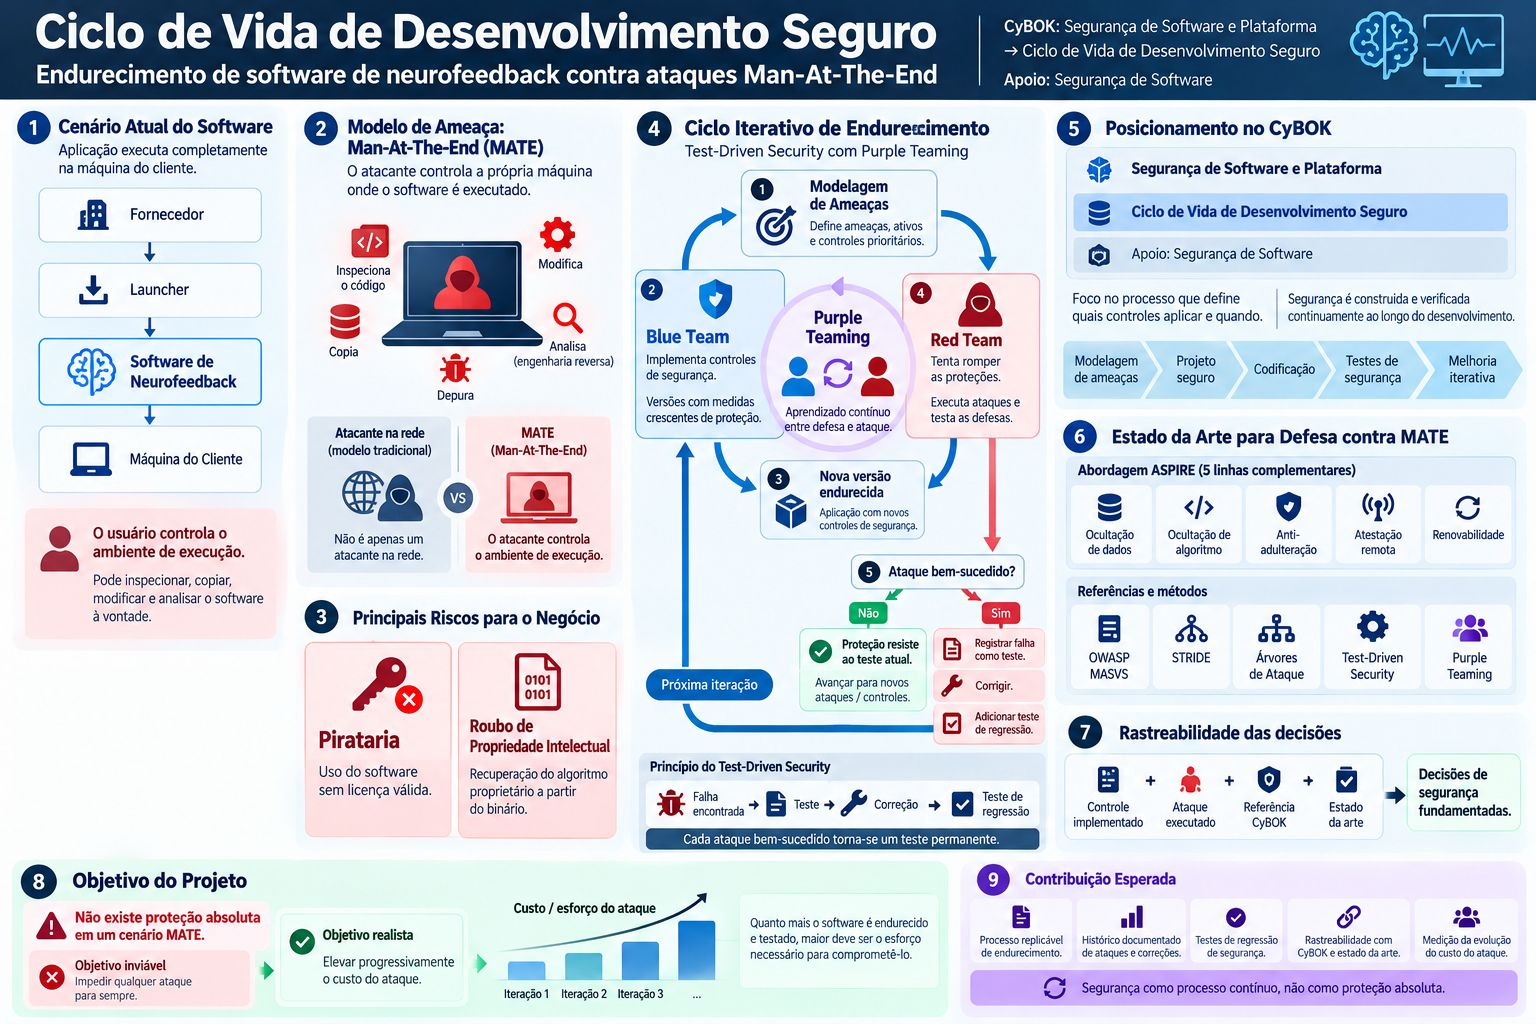
\includegraphics[width=\textwidth]{infografico.jpg}
\caption{Visão geral do projeto: cenário, modelo de ameaça, riscos, ciclo iterativo red e blue, posicionamento no CyBOK, estado da arte e objetivo.}
\label{fig:infografico}
\end{figure}

O resultado medido ao longo das cinco builds, em resumo, foi o seguinte. Para a pirataria, o ataque mais barato que funcionava custou 5 minutos na v0 e deixou de existir na v3 e na v4: nenhum caminho conhecido funcionou, e o red team gastou até 45 minutos sem sucesso numa mesma build. Para o roubo do algoritmo, o custo do caminho completo mais barato dobrou, de 5 para 10 minutos, mas a árvore de ataque seguiu aberta, porque o algoritmo continua executando na máquina do atacante. Em uma frase: dá para tornar a pirataria cara demais para valer a pena; o algoritmo dá para encarecer, mas não para esconder.

O restante do relatório percorre os artefatos do repositório na ordem em que foram produzidos. A Seção~\ref{sec:fundamentacao} apresenta a fundamentação e o estado da arte, e a Seção~\ref{sec:objeto} descreve o aplicativo e o mock usado no lugar dele. As Seções~\ref{sec:ameacas} a~\ref{sec:arvores} cobrem a modelagem de ameaças, os casos de abuso e as árvores de ataque. A Seção~\ref{sec:processo} detalha o processo, a suíte de testes e a esteira, e a Seção~\ref{sec:rastreabilidade}, a matriz de rastreabilidade. A Seção~\ref{sec:iteracoes} narra as cinco iterações, a Seção~\ref{sec:resultados} reúne os resultados, a Seção~\ref{sec:discussao} os discute e a Seção~\ref{sec:conclusao} conclui. O Apêndice~\ref{ap:custos} transcreve o registro completo de custo.

\section{Fundamentação e estado da arte}
\label{sec:fundamentacao}

\subsection{O CyBOK e o ciclo de vida de desenvolvimento seguro}

O CyBOK organiza o conhecimento de cibersegurança em áreas de conhecimento agrupadas em categorias \parencite{cybok2021}. O problema deste trabalho se situa na categoria de Segurança de Software e Plataforma, na área de Ciclo de Vida de Desenvolvimento Seguro (Secure Software Lifecycle) \parencite{williams2021}, com apoio da área de Segurança de Software.

Essa área parte da premissa de que segurança não é uma funcionalidade acrescentada ao final, e sim uma propriedade construída e verificada continuamente ao longo do desenvolvimento. Suas características centrais são a modelagem de ameaças no início, a incorporação de práticas seguras no projeto e na codificação, o teste de segurança como atividade recorrente e a melhoria iterativa a cada ciclo. Ela se distingue da área vizinha de Segurança de Software, que foca em categorias concretas de falhas de código, por tratar do processo que decide quais controles aplicar e quando. Distingue-se das dimensões de Segurança de Sistemas e de Infraestrutura por não ser sobre um mecanismo isolado (criptografia, hardware, rede), mas sobre como conduzir o desenvolvimento. E separa-se da dimensão de Ataques e Defesas por atuar na fase de construção, e não na operação e na resposta a incidentes.

A área descreve processos prescritivos de ciclo de vida seguro, entre eles o Security Development Lifecycle (SDL) da Microsoft \parencite{howard2006}, os pontos de contato (Touchpoints) de \textcite{mcgraw2006} e as práticas fundamentais da SAFECode \parencite{safecode2018}, além das adaptações desses processos a contextos como o desenvolvimento ágil e o DevOps. Práticas comuns a esses processos, como modelagem de ameaças, casos de abuso, requisitos de segurança, métricas, padrões de criptografia, gestão de componentes de terceiros, análise estática e teste de penetração, aparecem ao longo deste trabalho e são apontadas onde entram. Três outras áreas do CyBOK dão apoio pontual: Segurança de Software, para as fraquezas do binário; Criptografia, para a licença assinada; e Autenticação, Autorização e Responsabilização, para o licenciamento.

\subsection{O atacante Man-At-The-End}

No modelo MATE, o atacante tem acesso físico e administrativo ao dispositivo em que o software executa \parencite{collberg2009}. Ele pode ler o binário, executá-lo sob um depurador, alterar a memória do processo, interceptar chamadas e reescrever o código. Contra esse atacante, nenhuma proteção que resida inteiramente no cliente é absoluta: com esforço suficiente, quem controla a máquina adultera o binário ou reconstrói o que ele faz. O que as defesas fazem é encarecer o ataque. Por isso a pergunta útil deixa de ser \enquote{o software é seguro?} e passa a ser \enquote{quanto custa atacá-lo, e esse custo supera o valor do que se protege?}.

\subsection{Proteção de software contra o MATE}

A proteção de software contra atacantes MATE conta com corpos de conhecimento consolidados. O projeto europeu ASPIRE organiza as defesas em cinco linhas complementares, ocultação de dados, ocultação de algoritmo, anti-adulteração, atestação remota e renovabilidade, e avalia a proteção pelo custo do ataque, não por um veredito binário de seguro ou inseguro \parencite{aspire}. O padrão OWASP MASVS, embora voltado a aplicativos móveis, traz uma categoria dedicada à resiliência contra engenharia reversa e adulteração, a MASVS-RESILIENCE, usada aqui por analogia: RESILIENCE-1 para integridade da plataforma, RESILIENCE-2 para anti-adulteração, RESILIENCE-3 para dificultar a análise estática e RESILIENCE-4 para dificultar a análise dinâmica \parencite{masvs}. As fraquezas são nomeadas pelo catálogo CWE \parencite{cwe}.

Uma lição central desse estado da arte orienta as expectativas: em um cenário MATE, ocultar um segredo que precisa executar no cliente é, no fim, segurança por obscuridade (CWE-656). A ofuscação e a compilação nativa encarecem a leitura, mas não a impedem. A mitigação que de fato derrota o MATE é não enviar o segredo ao cliente.

\subsection{Métodos de engenharia de segurança}

A condução do processo se apoia em métodos estabelecidos. A modelagem de ameaças usa o STRIDE \parencite{shostack2014}, que classifica ameaças em falsificação de identidade (Spoofing), adulteração (Tampering), repúdio (Repudiation), vazamento de informação (Information disclosure), negação de serviço (Denial of service) e elevação de privilégio (Elevation of privilege). Os casos de abuso descrevem o comportamento do sistema sob um ator malicioso, o oposto das histórias de usuário \parencite{sindre2005,mcgraw2006}. As árvores de ataque organizam os caminhos que um atacante pode percorrer até um objetivo, com nós OR, em que basta um caminho, e AND, em que todos são necessários \parencite{schneier1999}. O Test-Driven Security leva para a segurança a lógica do desenvolvimento guiado por testes: o controle nasce junto com um teste que prova que ele funciona e que, dali em diante, impede a volta da falha \parencite{vehent2018}. O purple teaming junta o time que ataca e o time que defende em torno do mesmo resultado, a cada ciclo.

\subsection{Princípios de projeto seguro}

O CyBOK retoma os princípios de projeto de \textcite{saltzer1975}. Três deles explicam boa parte das decisões e do resultado deste trabalho. O padrão seguro em caso de falha (fail-safe defaults) orientou as respostas de integridade, que fecham o treino quando falta qualquer evidência de que o pacote está íntegro. A separação de privilégio orientou as duas guardas independentes e a chave privada do fornecedor fora do cliente. E o projeto aberto (open design), segundo o qual a segurança não deve depender do segredo do mecanismo, antecipa a diferença entre as duas histórias: a licença não depende de esconder nada no cliente, e fechou; o algoritmo depende, e só encareceu.

\section{O objeto: o aplicativo e o mock}
\label{sec:objeto}

\subsection{O aplicativo real}

O produto real é um aplicativo de desktop para Windows, em Avalonia~11.3 sobre .NET~10, organizado em MVVM com o CommunityToolkit.Mvvm. A leitura de EEG vem de um sensor BrainBit Flex~4, conectado por Bluetooth Low Energy e acessado pelo SDK do fabricante (XNeuroSDK). Todo o processamento, do sinal bruto ao índice de feedback, acontece localmente, por um pipeline proprietário de processamento digital de sinais (DSP), que é o ativo de propriedade intelectual da empresa. O aplicativo é distribuído por instalador, sem atualização automática, e no início do trabalho não tinha verificação de licença robusta, verificação de integridade nem qualquer proteção do algoritmo. A hardkey de licença que aparece nas árvores de ataque pertence ao software legado da empresa; o aplicativo novo partiu do zero.

\subsection{Por que um mock}

O repositório é público, e o algoritmo real não pode ser exposto. Por isso o aplicativo atacado neste trabalho é um mock: uma aplicação figurada com a mesma arquitetura e as mesmas superfícies de ataque do produto real, mas com o núcleo de processamento de sinal substituído por um stub sem valor comercial. A escolha preserva o que importa para o trabalho, isto é, licença, integridade do binário, arquivos locais, execução e leitura do algoritmo, sem expor a propriedade intelectual. Quando o processo estiver validado, basta trocar o stub pelo módulo real num ambiente fechado da empresa, e os controles já vêm testados.

Há um cuidado registrado no próprio repositório: o stub precisa ter complexidade parecida com a do real no ponto que a defesa protege. Para medir a ocultação de algoritmo, um \texttt{return input} não serviria, porque a conclusão não se transferiria ao produto. O stub implementa um algoritmo de verdade, com filtros, transformada rápida de Fourier, índice por bandas e limiar adaptativo, e o sensor é simulado com sinal sintético.

\subsection{Estrutura do mock}

O código fica em \texttt{app/}, numa solução com quatro projetos e uma pasta de ferramentas, descrita no Quadro~\ref{qd:mock}. A mesma linha de versões do produto real foi mantida (Avalonia~11.3, CommunityToolkit.Mvvm~8.4 e xunit.v3~3.2), no patch mais recente de cada uma. Um \texttt{Directory.Build.props} fixa o que vale para todos os projetos: .NET~10, auditoria de pacotes no restore, em que uma vulnerabilidade moderada ou pior quebra o build, e build de Release sem PDB, como o pacote entregue à clínica.

\begin{table}[htbp]
\centering
\caption{Estrutura do mock em \texttt{app/}.}
\label{qd:mock}
\small
\begin{tabular}{L{4.2cm}L{10.4cm}}
\toprule
Projeto & Papel \\
\midrule
\texttt{NeuroMock} & App Avalonia (WinExe): barreira de licença, tela de treino, tela de ativação, guardas e respostas de integridade. \\
\texttt{NeuroMock.Core} & Lógica pura, sem Avalonia: licenciamento, integridade (manifesto), processamento (stub de DSP), sensor (sinal sintético) e sessão (CSV local). \\
\texttt{NeuroMock.Fornecedor} & Lado do fornecedor, fora do pacote: par de chaves, emissão de licença e assinatura do pacote. \\
\texttt{NeuroMock.Tests} & Testes funcionais do Core, da emissão e do manifesto (xunit.v3). \\
\texttt{ferramentas/} & Emissor de licença, assinador do pacote e, a partir da v3, o ofuscador do algoritmo. \\
\bottomrule
\end{tabular}
\end{table}

\subsection{Distribuição e reprodutibilidade}

O canal de distribuição do mock é o zip win-x64 que a esteira publica em cada tag \texttt{v*}, acompanhado do SHA-256. É o único alvo válido para o red team, que confere o hash antes de atacar. O instalador do produto real ficou fora das iterações, porque nenhuma folha das árvores depende dele. A reprodutibilidade vem de versões fixadas: o \texttt{global.json} fixa o SDK e o \texttt{dotnet-tools.json}, as ferramentas, com as mesmas versões no devcontainer (Linux, para higiene e análise automatizada) e na esteira. O ataque exploratório acontece na máquina pessoal de cada atacante, fiel ao modelo MATE, e a regressão automatizada roda num runner Windows, a mesma plataforma do alvo.

\section{Modelagem de ameaças}
\label{sec:ameacas}

O primeiro artefato do processo é a modelagem de ameaças (\texttt{docs/01-threat-model.md}). Ela corresponde à prática de modelagem de ameaças do SDL \parencite{howard2006} e à análise de risco arquitetural dos Touchpoints \parencite{mcgraw2006}, e foi feita uma vez, no início, para derivar e justificar o escopo.

\subsection{Cenário e fluxo de dados}

O software executa inteiramente na máquina do cliente, e o modelo de atacante é o MATE: o adversário controla o próprio ambiente de execução e pode inspecionar, copiar e alterar o binário. A premissa que orienta todo o trabalho já aparece aqui: contra quem controla a máquina não há proteção absoluta, e o objetivo é elevar o custo do ataque acima do valor do ativo. A Figura~\ref{fig:dfd} mostra o diagrama de fluxo de dados com as fronteiras de confiança, isto é, os pontos em que o controle do fornecedor termina.

\begin{figure}[htbp]
\centering
\begin{tikzpicture}[
  caixa/.style={draw, rounded corners=2pt, align=center, font=\small, text width=3.4cm, minimum height=1.1cm, inner sep=3pt, fill=white},
  seta/.style={-{Stealth[length=2.2mm]}, thick},
  dupla/.style={{Stealth[length=2.2mm]}-{Stealth[length=2.2mm]}, thick}
]
\node[caixa] (inst) at (0,3.4) {Instalador\\canal de distribuição};
\node[caixa] (app) at (-4.4,0) {App Avalonia\\telas e portão de licença};
\node[caixa] (core) at (0,0) {Core\\licença, integridade e DSP};
\node[caixa] (arq) at (4.4,0) {Arquivos locais\\licença e sessão};
\node[font=\small\bfseries, anchor=south west] (rotulo) at (-6.2,0.75) {F1: máquina do cliente, território do atacante};
\node[draw, dashed, rounded corners=4pt, inner sep=8pt, fit=(app)(core)(arq)(rotulo)] (f1) {};
\node[caixa] (sensor) at (0,-3.4) {Sensor EEG\\BrainBit Flex 4};
\draw[seta] (inst) -- node[right, font=\footnotesize] {instala (F2)} (f1.north);
\draw[dupla] (app) -- (core);
\draw[dupla] (core) -- (arq);
\draw[dupla] (f1.south) -- node[right, font=\footnotesize] {Bluetooth LE (F3)} (sensor);
\end{tikzpicture}
\caption{Diagrama de fluxo de dados e fronteiras de confiança.}
\label{fig:dfd}
\end{figure}

As fronteiras de confiança são três:
\begin{itemize}
\item \textbf{F1, a máquina do cliente}: território hostil. Quem instala tem permissão de administrador e pode ler e adulterar tudo: o binário, os arquivos locais e a memória do processo.
\item \textbf{F2, o canal de distribuição}: de onde o aplicativo é obtido. Sem verificação de assinatura, vira vetor de cadeia de suprimentos. No produto real, o instalador não tem atualização automática, o que também significa que versões antigas continuam circulando.
\item \textbf{F3, o Bluetooth do EEG}: enlace entre o aplicativo e o sensor, passível de interceptação e de injeção.
\end{itemize}

\subsection{STRIDE por elemento}

O STRIDE foi aplicado a cada elemento do diagrama para derivar e justificar o escopo, não como atividade paralela. O Quadro~\ref{qd:stride} resume o resultado. A escala de risco é qualitativa: o impacto no negócio, pesado pelo que o atacante consegue fazer tendo a máquina na mão.

\begin{table}[htbp]
\centering
\caption{STRIDE por elemento do fluxo de dados, com risco qualitativo.}
\label{qd:stride}
\small
\setlength{\tabcolsep}{4pt}
\begin{tabular}{L{2.6cm}ccccccL{3.8cm}}
\toprule
Elemento & S & T & R & I & D & E & Observação \\
\midrule
App (binário) & -- & Alto & -- & Alto & baixo & baixo & patch de licença; extração do algoritmo \\
Arquivos locais & -- & Médio & -- & médio & baixo & -- & licença e sessão em claro \\
Instalador e canal & Médio & Médio & -- & baixo & baixo & -- & instalador ou atualização maliciosos \\
Bluetooth do EEG & baixo & baixo & -- & baixo & baixo & -- & sinal de um sensor isolado, de baixo valor \\
\bottomrule
\end{tabular}
\par\smallskip
{\footnotesize S: Spoofing; T: Tampering; R: Repudiation; I: Information disclosure; D: Denial of service; E: Elevation of privilege.}
\end{table}

O risco residual se concentra em Tampering e Information disclosure sobre o binário, que viram as duas histórias de atacante: adulterar o aplicativo para pular a licença e ler o algoritmo. Os demais vetores têm baixo valor neste produto: a leitura de EEG de um sensor isolado, sem contexto clínico, diz pouco por si.

\subsection{Adversários e escopo}

Ameaça sem adversário é paranoia sem foco. O trabalho considera dois perfis, que geram as duas histórias. A \textbf{clínica pirata} quer usar o software sem pagar; tem motivação econômica e habilidade baixa a média, e gera a história de pirataria. O \textbf{concorrente} quer o algoritmo proprietário de processamento de sinal; tem habilidade alta, e gera a história de roubo de propriedade intelectual.

Duas classes de ameaça ficaram fora do escopo, por decisão registrada no início do projeto: o insider que fuça dados de paciente, porque o dado de EEG de um sensor isolado tem baixo valor por si, e os ataques de rede clássicos, como o homem no meio, porque o software é local. O modelo também registra uma pendência de revisão: o produto real tem um canal local (loopback) de integração com jogos, que deve entrar no diagrama como superfície conhecida e fora de escopo.

\section{Casos de abuso: as histórias do atacante}
\label{sec:abuso}

O segundo artefato (\texttt{docs/02-abuse-cases.md}) transforma o resultado do STRIDE em histórias do atacante. Casos de abuso descrevem o comportamento do sistema sob um ator malicioso, o oposto das histórias de usuário \parencite{sindre2005,mcgraw2006}: cada ator mau recebe um objetivo e os caminhos que gostaria de percorrer, e as mitigações viram requisitos de segurança que alimentam a árvore de ataque e a suíte de testes. É a prática de casos de abuso e de requisitos de segurança dos Touchpoints \parencite{mcgraw2006}.

\subsection{AC-1: pirataria}

\begin{quote}
\textbf{Como} clínica pirata, \textbf{quero} executar o software sem uma licença válida, \textbf{para} não pagar pelo produto.
\end{quote}

\begin{itemize}
\item \textbf{Ator}: clínica pirata, com motivação econômica e habilidade baixa a média.
\item \textbf{Ativo alvo}: a verificação de licença.
\item \textbf{Gatilho}: o aplicativo roda localmente, então todo o mecanismo de licença está na mão do atacante.
\item \textbf{Caminhos desejados}: adulterar o binário para pular a verificação (patch no IL, anulação do salto condicional); manipular a verificação em tempo de execução (depurador, hook, edição de memória); forjar ou reusar o artefato de licença (copiar de outra máquina, keygen, editar em claro); contornar uma ativação online, se adotada (emular o servidor, replay); derrotar uma hardkey, se adotada (emular ou clonar o dongle).
\item \textbf{Requisito de segurança derivado}: o aplicativo deve recusar execução sem licença válida, e a verificação deve resistir a adulteração estática e dinâmica dentro do custo-alvo.
\item \textbf{Critério de aceite}: rodar o aplicativo com cada técnica acima deve resultar em recusa de execução, verificada pela suíte de regressão.
\end{itemize}

\subsection{AC-2: roubo do algoritmo proprietário}

\begin{quote}
\textbf{Como} concorrente, \textbf{quero} recuperar o pipeline proprietário de processamento de sinal a partir do binário, \textbf{para} replicá-lo no meu produto.
\end{quote}

\begin{itemize}
\item \textbf{Ator}: concorrente, com habilidade alta.
\item \textbf{Ativo alvo}: o algoritmo de processamento de sinal, substituído no repositório por um stub.
\item \textbf{Gatilho}: um binário .NET descompila com facilidade, porque o IL é quase legível como código-fonte.
\item \textbf{Caminhos desejados}: descompilar o assembly e ler o algoritmo diretamente; localizar o módulo do algoritmo e compreendê-lo, um nó AND em que é preciso localizar e compreender; extrair pesos e parâmetros de configuração.
\item \textbf{Requisito de segurança derivado}: elevar o custo de localizar e compreender o algoritmo e, como recomendação arquitetural, avaliar mover o núcleo sensível para fora do cliente.
\item \textbf{Critério de aceite}: medir o tempo que o red team leva para extrair o algoritmo a cada iteração. A meta é a curva de custo subir.
\end{itemize}

O próprio caso de abuso registra uma nota honesta, escrita antes de qualquer build: a única mitigação que de fato derrota o MATE aqui é não enviar o segredo, movendo o pipeline para um servidor. Mantendo tudo local, ofuscação e compilação nativa são endurecimento parcial, não solução. A nota não é uma falha do trabalho, e sim um achado; as iterações a confirmaram com números (Seção~\ref{sec:resultados}).

\subsection{Casos fora de escopo}

Ficaram registrados para rastreabilidade, mas fora do escopo acordado, o vazamento de dados de paciente, de baixo valor neste cenário, e os ataques de rede, porque o software é local.

\section{Árvores de ataque}
\label{sec:arvores}

O terceiro artefato (\texttt{docs/03-attack-trees.md}) desdobra cada caso de abuso numa árvore de ataque \parencite{schneier1999}. A árvore é o mapa do território, não o roteiro do jogo: lista os caminhos conhecidos para o objetivo do atacante. A raiz é o objetivo e as folhas são ataques concretos e executáveis; um conector OR significa que basta um caminho, e um AND, que todos os filhos são necessários. Cada folha vira um teste de regressão com o nome dela (por exemplo, T-F1.2) e tem um estado avaliado a cada build: \emph{aberta}, quando o ataque tem sucesso, ou \emph{fechada}, quando o controle resiste. A árvore não muda entre as builds; o que muda é a coluna de estados, que deve ficar mais fechada a cada iteração.

\subsection{Árvore 1: usar o aplicativo sem licença válida}

A Figura~\ref{fig:arvore1} reproduz o diagrama da árvore 1 que está no repositório, desenhado no início do projeto com o estado da build 0, e o Quadro~\ref{qd:arvore1} lista as folhas.

\begin{figure}[htbp]
\centering
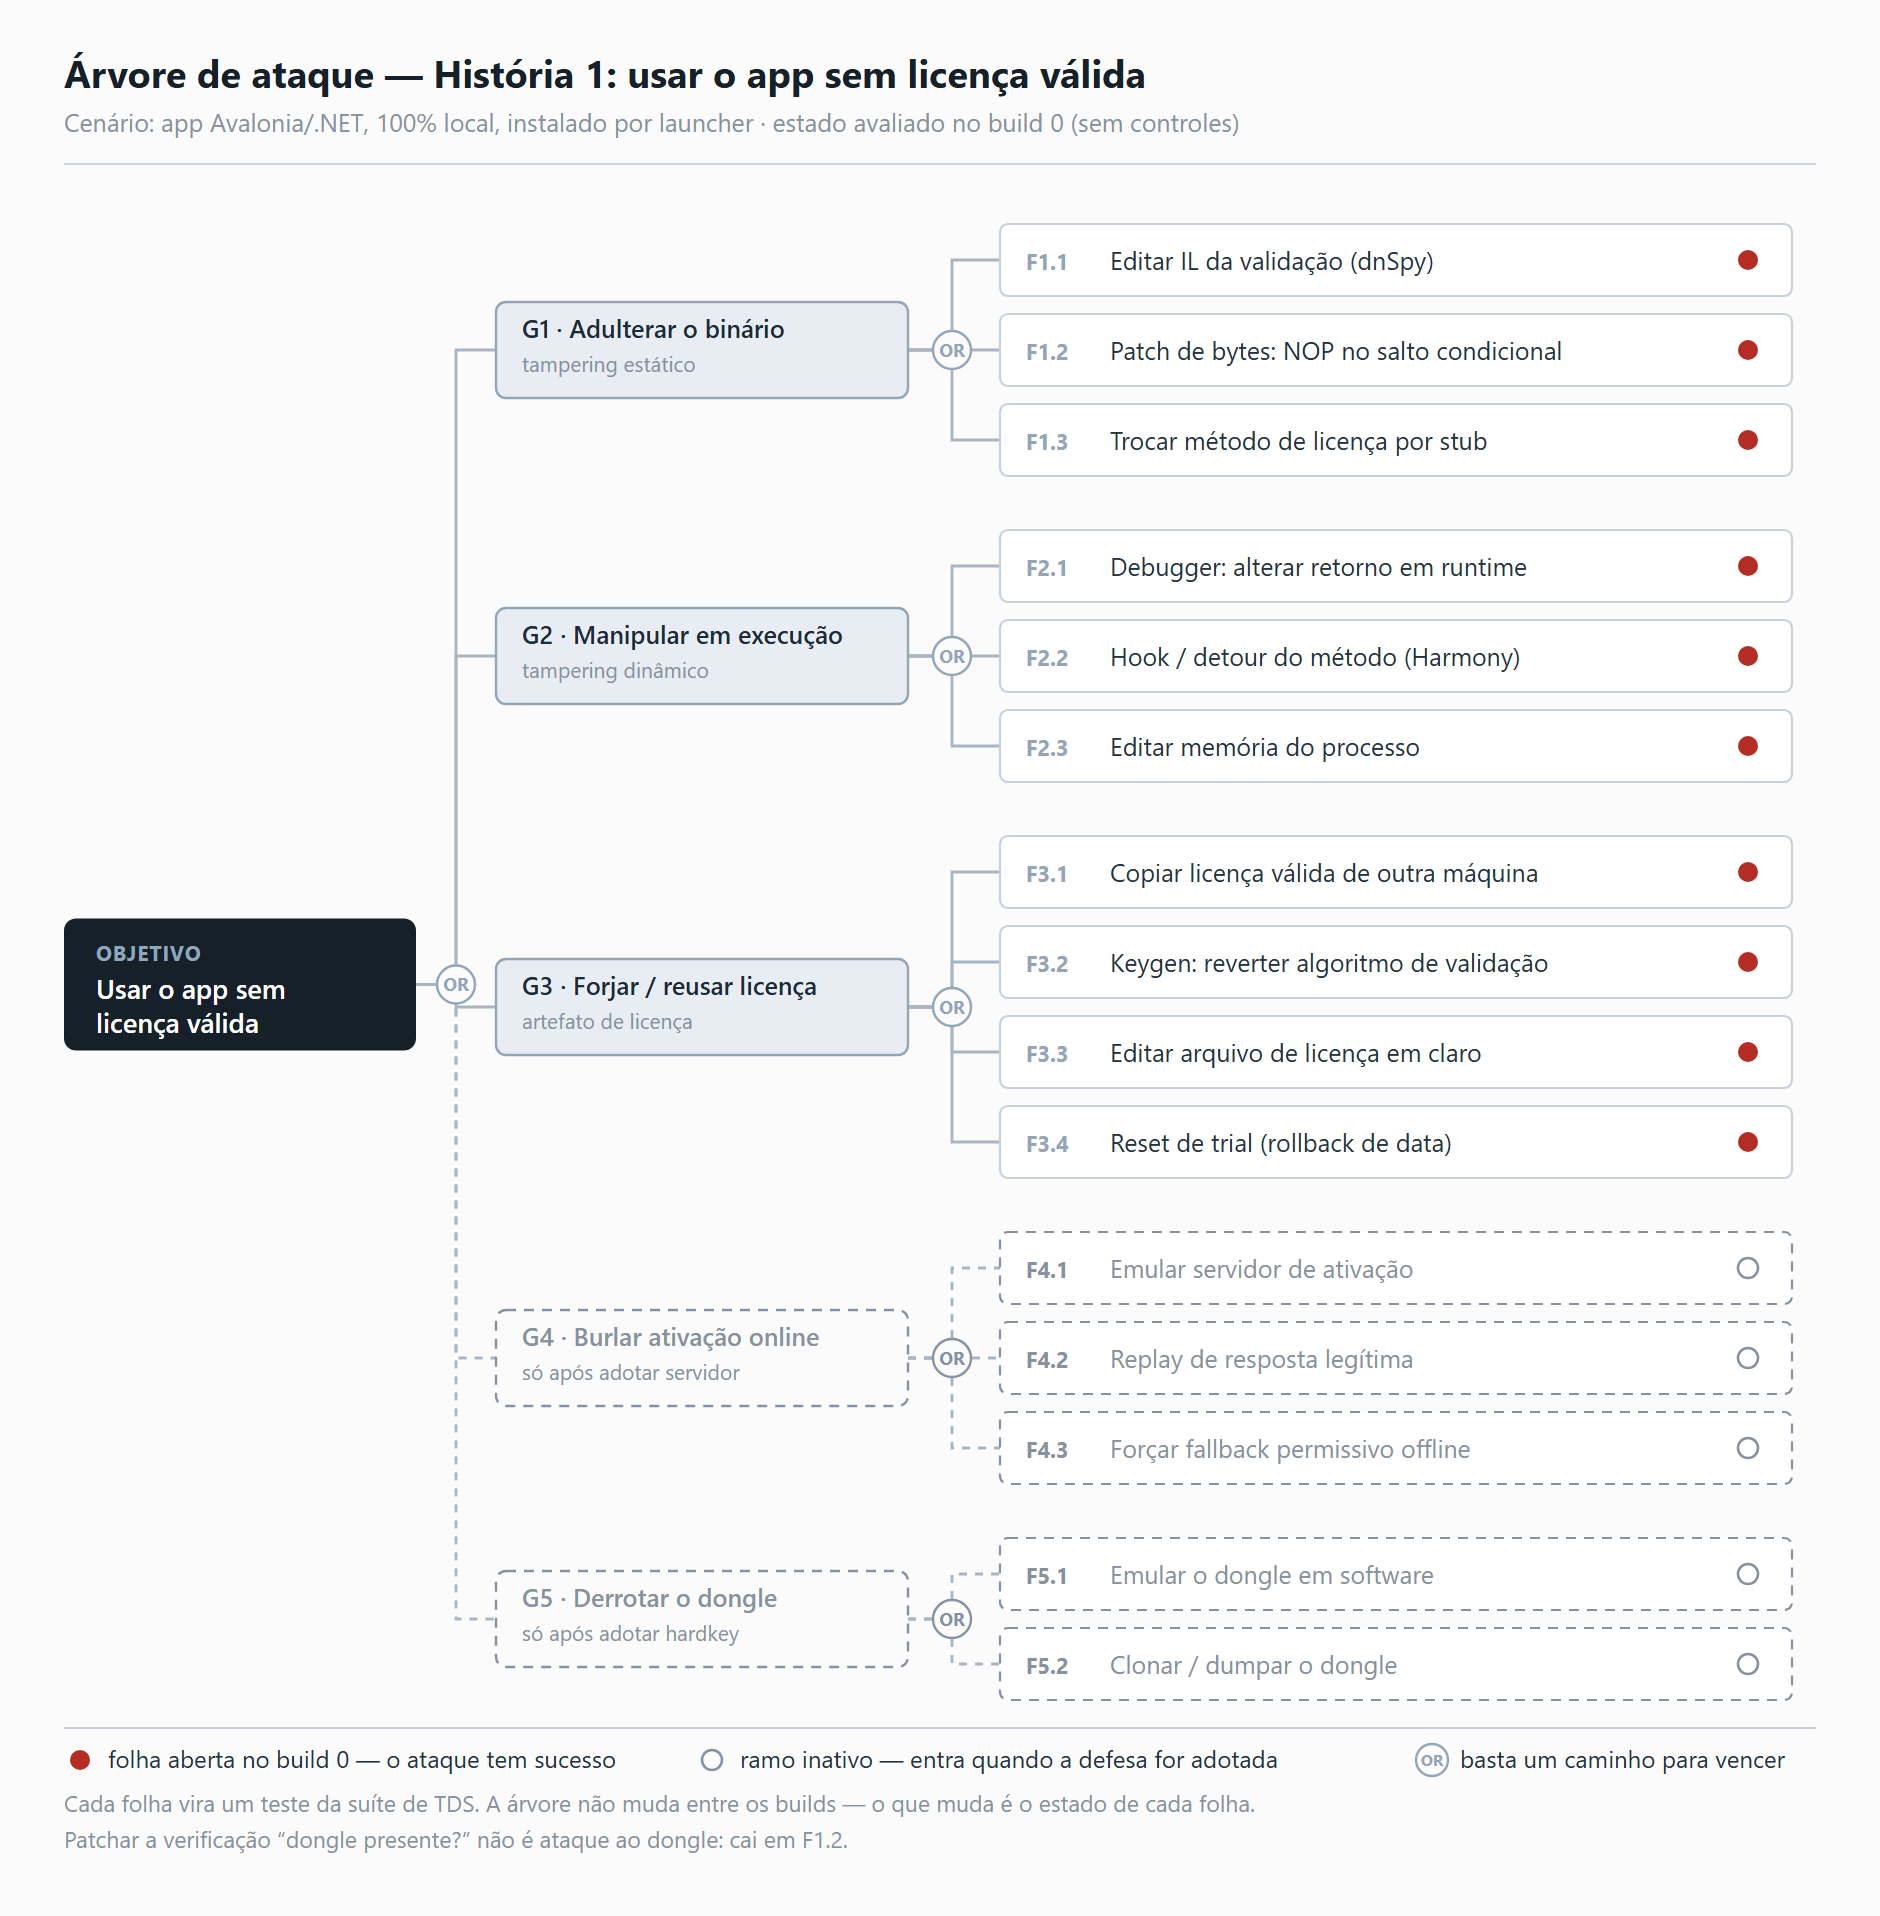
\includegraphics[width=0.92\textwidth]{arvore-ataque-1.png}
\caption{Árvore de ataque da história 1, no estado da build 0, como desenhada no início do projeto. Depois, a folha F3.4 ficou inativa, porque o mock não tem período de avaliação.}
\label{fig:arvore1}
\end{figure}

\begin{table}[htbp]
\centering
\caption{Folhas da árvore 1 (raiz OR).}
\label{qd:arvore1}
\small
\begin{tabular}{L{4.4cm}L{1.2cm}L{8.8cm}}
\toprule
Ramo & Folha & Ataque \\
\midrule
G1, adulterar o binário (tampering estático, OR) & F1.1 & Editar o IL da validação (dnSpy, ILSpy) e salvar o assembly \\
 & F1.2 & Patch de bytes: NOP no salto condicional \\
 & F1.3 & Substituir o método de licença por um stub que sempre libera \\
\midrule
G2, manipular em execução (tampering dinâmico, OR) & F2.1 & Depurador: alterar o retorno da validação em runtime \\
 & F2.2 & Hook ou detour do método (por exemplo, Harmony) \\
 & F2.3 & Editar a memória do processo (flag de licenciado) \\
\midrule
G3, forjar ou reusar a licença (OR) & F3.1 & Copiar uma licença válida de outra máquina \\
 & F3.2 & Keygen: reverter o algoritmo de validação \\
 & F3.3 & Editar o arquivo de licença em claro \\
 & F3.4 & Reset do período de avaliação (inativa: o mock não tem trial) \\
\midrule
G4, contornar ativação online (inativo) & F4.1 a F4.3 & Emular o servidor, replay de resposta legítima, forçar o modo offline permissivo \\
\midrule
G5, derrotar a hardkey (inativo) & F5.1 e F5.2 & Emular o dongle em software, clonar o conteúdo do dongle \\
\bottomrule
\end{tabular}
\end{table}

A árvore ensina duas coisas antes de qualquer ataque. Primeiro, enquanto o binário puder ser adulterado (G1 e G2), qualquer sofisticação em G3, G4 ou G5 é contornável por cima: patchear a verificação \enquote{a licença é válida?} não é atacar a licença, é cair em F1.2. A raiz real do problema é a integridade do binário. Segundo, G4 e G5 nascem inativos: só entram em jogo quando o blue team adotar aquele controle, mas os caminhos já estão desenhados de antemão.

\subsection{Árvore 2: recuperar o algoritmo proprietário}

\begin{table}[htbp]
\centering
\caption{Folhas da árvore 2 (raiz OR).}
\label{qd:arvore2}
\small
\begin{tabular}{L{4.4cm}L{1.2cm}L{8.8cm}}
\toprule
Ramo & Folha & Ataque \\
\midrule
H1, leitura direta (OR) & H1.1 & Descompilar o assembly e ler o algoritmo \\
 & H1.2 & Extrair parâmetros e pesos de configuração \\
\midrule
H2, compreender o algoritmo localizado (AND) & H2.1 & Localizar o módulo do algoritmo no binário \\
 & H2.2 & Compreender a lógica: nomes, fluxo e matemática \\
\bottomrule
\end{tabular}
\end{table}

O ramo H2 é um nó AND: para roubar de forma útil, o atacante precisa localizar e compreender. É exatamente onde a ofuscação atua, encarecendo H2.2. Na medição, o red vence a árvore 2 quando entrega uma reimplementação que reproduz a saída do stub num sinal de entrada que não viu, um oráculo. E, por ser AND, o custo de um caminho por H2 é a soma de localizar e compreender: localizar sozinho não rouba nada. A árvore também registra o teto honesto do MATE: nenhuma folha dela fecha em definitivo enquanto o algoritmo estiver no cliente.

Somando as duas árvores, são 13 folhas ativas (F1.1 a F1.3, F2.1 a F2.3, F3.1 a F3.3, H1.1, H1.2, H2.1 e H2.2) e três ramos ou folhas inativos até que o controle correspondente exista (F3.4, G4 e G5).

\section{O processo: Test-Driven Security com red e blue team}
\label{sec:processo}

Os artefatos de processo descrevem como os ciclos rodam na prática: o ciclo em si (\texttt{docs/05-tds-process.md}); o plano das iterações, com calendário, ritual, regras de engajamento e medição de custo (\texttt{docs/06-plano-iteracoes.md}); o passo a passo do red team (\texttt{docs/07-guia-red-team.md}); e o fluxo de branches e de pull requests (\texttt{CONTRIBUTING.md}). Juntos, eles são a parte mais reutilizável do trabalho: nada neles depende de neurofeedback.

\subsection{O ciclo}

O ciclo tem quatro momentos. O primeiro é a \textbf{modelagem}, feita uma vez: o STRIDE sobre o fluxo de dados deriva as histórias, cada história vira uma árvore, e cada folha vira um teste. O segundo é a \textbf{build 0}, o aplicativo sem controles, de propósito, como linha de base; quase todas as folhas ficam abertas. O terceiro é a \textbf{iteração}, repetida: o red ataca a build atual seguindo as árvores; cada ataque com sucesso vira uma issue com evidência; o blue implementa o controle num pull request que inclui o teste de regressão; e o teste passa a rodar em todo build futuro. O quarto é o \textbf{fim}, quando o custo de fechar as folhas restantes passa do valor de fechá-las. No MATE sempre sobra folha aberta, e isso é documentado como conclusão, não como fracasso.

Os papéis são dois: o blue team construiu as builds e os controles, e o red team atacou e manteve as árvores e os casos de abuso. A regra de ouro do repositório resume a disciplina: nenhuma defesa entra na \texttt{main} sem o teste de regressão correspondente, porque segurança é regra da esteira, não disciplina individual. Controles estruturais, como hardkey, servidor de ativação ou o algoritmo no servidor, são avaliados como experimentos numa branch \texttt{hipotese/<nome>}: o blue implementa, o red ataca a branch, e só sobe para a \texttt{main} o que se prova. As demais branches seguem o mesmo vocabulário: \texttt{fix/<folha>} para as correções do blue e \texttt{ataque/<folha>} para os testes do red.

\subsection{Como um ataque vira teste sem travar a main}

No MATE sempre sobra folha aberta. Se o teste de uma folha aberta simplesmente falhasse, a esteira nunca ficaria verde e a proteção de branch travaria a \texttt{main} para sempre. Por isso cada folha tem um estado declarado em \texttt{security-tests/estado-folhas.json}, e cada teste compara o resultado do ataque com esse estado, como mostra o Quadro~\ref{qd:estado}.

\begin{table}[htbp]
\centering
\caption{O teste compara o resultado do ataque com o estado declarado da folha.}
\label{qd:estado}
\small
\begin{tabular}{L{2.8cm}L{2.6cm}L{2.2cm}L{6.4cm}}
\toprule
Estado declarado & O ataque & Esteira & Significado \\
\midrule
aberta & funcionou & verde & buraco conhecido e documentado \\
aberta & falhou & vermelha & a folha fechou: atualizar o estado e a matriz \\
fechada & falhou & verde & o controle resiste \\
fechada & funcionou & vermelha & regressão: o merge é barrado \\
\bottomrule
\end{tabular}
\end{table}

O desenvolvimento guiado por testes acontece em quatro passos. O red sobe o teste com a folha \texttt{aberta}: a esteira fica verde e o buraco fica registrado. O blue abre uma branch \texttt{fix/<folha>}, cujo primeiro commit muda a folha para \texttt{fechada}, e a esteira fica vermelha. O controle entra, e a esteira volta ao verde. Depois do merge, se a folha reabrir em qualquer build, a esteira acusa a regressão.

Dois cuidados impedem resultados enganosos. O primeiro é o \textbf{controle positivo}: antes de cada ataque, o teste confirma que o aplicativo original recusa sem licença e abre o treino com uma licença legítima. A partir da v1, essa licença é emitida na hora para a máquina que roda a suíte, com a chave privada do fornecedor guardada como segredo da esteira; sem a chave, fora da esteira, o controle fica parcial. Se o controle positivo falhar, o resultado é inconclusivo, nunca \texttt{fechada}: um build quebrado que nem abre não pode parecer seguro. O segundo é a \textbf{observação de fora}: o teste observa o aplicativo como o atacante observaria, rodando o executável e verificando se a janela principal abriu e, desde a v2, se continuou aberta durante 30 segundos. Não existe flag ou modo de teste dentro do binário, que seria superfície de ataque a mais.

\subsection{A suíte de testes de ataque}

A suíte (\texttt{security-tests/}) é um projeto xunit.v3 em C\#, com a biblioteca dnlib, a mesma de manipulação de assembly do dnSpy, para os patches. Cada teste é um procedimento repetível com resultado passa ou falha: executa a técnica da folha contra uma cópia do zip da release, observa de fora e compara com o estado declarado. O harness tem quatro peças: \texttt{Alvo.cs} extrai o zip, dá uma cópia descartável por teste, roda e observa o aplicativo; \texttt{EstadoFolhas.cs} compara o resultado com o estado declarado; \texttt{ControlePositivo.cs} garante que o alvo original funciona; e \texttt{Assembleia.cs} abre, altera e grava um assembly. O que o atacante sabe do alvo, como nomes e offsets, vem da tentativa em caixa preta e fica no teste, não no harness. O ponto de entrada é o \texttt{run-all.ps1}, o mesmo na esteira e na máquina de cada um.

Ao fim das cinco builds, a suíte tinha 13 testes de ataque, além do controle positivo: T-F1.1, T-F1.2, T-F1.3, T-F2.2, T-F3.1, T-F3.2 e T-F3.3 (estes dois também na forma da v1), T-H1.1, T-H1.2, T-H2.1 e T-H2.2. As folhas F2.1 (depurador) e F2.3 (edição de memória) foram medidas na mão, porque são difíceis de automatizar na esteira; o custo foi para o registro, e a matriz anota que elas não têm regressão automática. Na v4, um guarda no harness (\texttt{CopiaDoAlvo.EhNativo}) passou a detectar o alvo nativo: os testes de folhas já fechadas que dependem de IL contam como neutralizados por construção, e os das folhas do algoritmo, ainda abertas, pulam e são medidos na mão.

\subsection{A esteira}

A esteira (\texttt{.github/workflows/security.yml}) roda a cada push e a cada pull request, em duas camadas, como mostra a Figura~\ref{fig:esteira}. A \textbf{camada de higiene}, em Linux, procura segredos vazados (gitleaks), faz análise estática (CodeQL), audita as dependências vulneráveis e roda os testes funcionais. A \textbf{camada de regressão MATE}, num runner Windows, gera o zip win-x64 da release e reaplica contra ele cada ataque conhecido. Em tag \texttt{v*}, a esteira publica a release com o SHA-256. A proteção de branch, configurada com rulesets do GitHub, exige pull request e os checks da esteira, bloqueia force push e impede mover ou apagar as tags.

\begin{figure}[htbp]
\centering
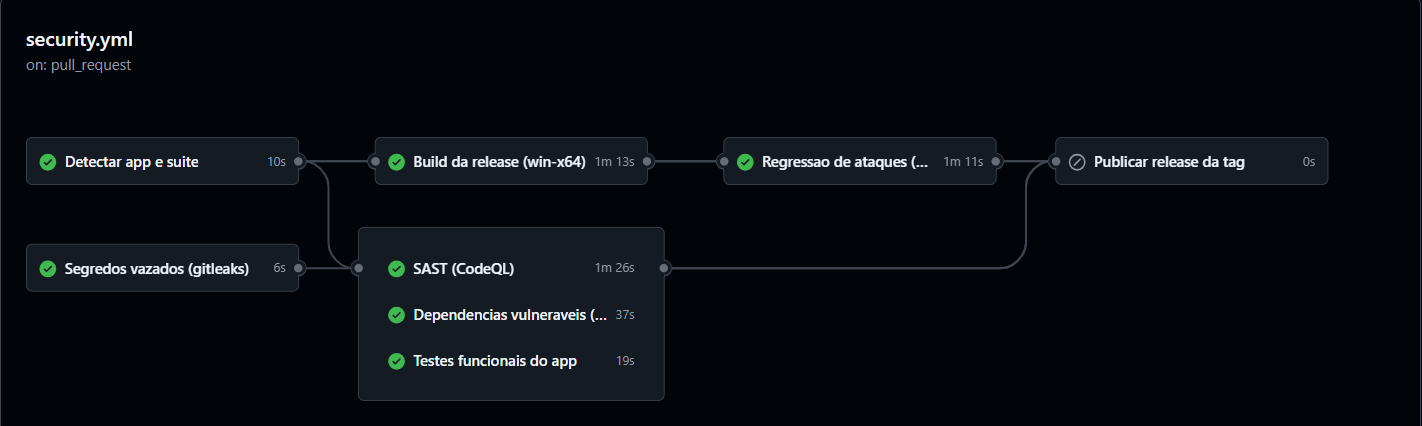
\includegraphics[width=\textwidth]{esteira-run.png}
\caption{Execução da esteira no GitHub Actions para um pull request de documentação (2 min 48 s, verde). A publicação da release só roda em tag.}
\label{fig:esteira}
\end{figure}

A chave privada do fornecedor, necessária para emitir a licença do controle positivo e para assinar o manifesto do pacote, existe na esteira só como o segredo \texttt{NEUROMOCK\_CHAVE\_PRIVADA}, e na máquina do blue fora de qualquer repositório. O risco ficou registrado: um colaborador com permissão de escrita conseguiria ler o segredo por um pull request que alterasse a esteira. Para um trabalho acadêmico, decidiu-se por um segredo simples; no produto real, a chave de emissão ficaria num ambiente com aprovação manual, ou fora da esteira de vez.

Essa organização cobre várias práticas que o CyBOK descreve nos processos prescritivos \parencite{williams2021,howard2006,safecode2018}: análise estática, gestão de componentes de terceiros, uso de ferramentas aprovadas e versões fixadas, e teste de segurança recorrente, adaptado ao DevOps. A gestão de terceiros teve efeito concreto: na v4, a auditoria de dependências barrou um compilador com vulnerabilidade conhecida, como mostra a Seção~\ref{sec:iteracoes}.

\subsection{Medição do custo de ataque}

O custo é a métrica principal do trabalho, por isso foi registrado desde a v0, numa linha por tentativa em \texttt{docs/metricas/custo-ataques.csv}, inclusive as que falharam: uma folha fechada sem tentativa registrada não prova nada. As colunas são data, build, folha, modo, atacante, ferramentas, minutos, resultado e evidência. O modo é \emph{preta}, quando o atacante usou só o artefato da release, ou \emph{branca}, quando consultou o código; o custo só vale para o MATE se o atacante não leu o código, então a caixa branca seria uma segunda medição, registrada à parte. O resultado é sucesso, falha ou timebox.

O timebox é de 2 horas por folha por build, e é um teto, não uma cota: folha que cai em minutos não consome o resto, e o teto só pesa nas que resistem. Ele foi mantido alto de propósito, porque com um teto baixo as builds finais virariam todas \enquote{mais de uma hora} e a curva de custo achataria onde deveria subir. A partir da v2, sucesso passou a ser usar o treino, não só vê-lo abrir: o red registra o resultado depois de deixar o treino aberto por pelo menos um minuto, e a regressão segue a mesma regra. Na árvore 2, o red vence quando entrega uma reimplementação que reproduz a saída do stub num sinal que não viu, e o tempo até lá é o custo.

\subsection{Regras de engajamento e guia do red team}

As regras de engajamento definem o jogo. O red ataca só o zip da release da tag, conferindo o SHA-256; ataca em caixa preta primeiro e só abre \texttt{app/} depois de registrar a tentativa; usa a própria máquina, fiel ao MATE; não ataca a infraestrutura (GitHub, esteira, máquinas dos colegas); e não commita binário adulterado, licença emitida por ele nem segredo, só scripts, passos e hashes.

O guia do red team transforma essas regras num passo a passo para cada ciclo: pegar o alvo e conferir o hash; atacar uma folha por vez dentro do timebox; registrar toda tentativa; abrir uma issue pelo modelo \enquote{Ataque}, com build, SHA-256, folha, modo, passos, evidência, custo e impacto; transformar a issue num teste numa branch \texttt{ataque/<folha>}, rodando a suíte localmente antes do pull request; e levar o resultado à reunião red/blue. O guia traz ainda um bloco de contexto pronto para o assistente de IA do red, que deixa claras as regras de caixa preta e de engajamento, e uma configuração opcional do Claude Code que nega a leitura de \texttt{app/}, para evitar a leitura acidental do código do alvo.

\subsection{Ritmo, ritual e build pronta}

O calendário foi organizado em torno dos encontros presenciais de terça e quinta, com um ciclo por encontro (Quadro~\ref{qd:calendario}). Para caber no prazo, o blue andou uma build à frente: quando o encontro começava, a build seguinte já estava pronta numa branch, e o encontro só consolidava. Se um ciclo atrasasse, a v4 viraria recomendação e a data final não se moveria.

\begin{table}[htbp]
\centering
\caption{Calendário dos ciclos.}
\label{qd:calendario}
\small
\begin{tabular}{L{2.4cm}L{1.4cm}L{1.4cm}L{8.6cm}}
\toprule
Encontro & Fecha & Lança & Testes do red que precisavam estar na \texttt{main} \\
\midrule
qui 05/11 & v0 & v1 & T-F3.1, T-F3.2 e T-F3.3 \\
ter 10/11 & v1 & v2 & T-F1.1, T-F1.2 e T-F1.3 \\
qui 12/11 & v2 & v3 & T-F2.x, T-H1.2 e T-H2.2 \\
ter 17/11 & v3 & v4 & T-H1.1 e T-H2.1 \\
qui 19/11 & v4 & nenhuma & consolidação final; depois, documentação e ensaio \\
\bottomrule
\end{tabular}
\end{table}

Cada encontro tem o mesmo ritual, a reunião red/blue, que é o momento \enquote{purple} do purple teaming: o red mostra o que funcionou, o que não funcionou e quanto custou; os testes do red entram na \texttt{main}; no pull request da build seguinte, as folhas que ela fecha viram \texttt{fechada}; e saem o merge, a coluna da build na matriz, a nota da iteração e a tag. Uma build só é entregue ao red quando a esteira está verde na \texttt{main}, a tag existe e a release foi publicada com o SHA-256, o estado de cada folha está declarado, a coluna da matriz está preenchida e existe a nota da iteração em \texttt{docs/iteracoes/}. Para caber no calendário, valeu ainda uma exceção registrada: se o teste de uma folha atrasasse, o blue podia escrevê-lo a partir dos passos da issue, depois de a tentativa em caixa preta estar registrada, porque a regra de o blue não escrever teste existe só para não revelar o alvo antes do ataque.

\section{A matriz de rastreabilidade}
\label{sec:rastreabilidade}

A matriz (\texttt{docs/04-controls-traceability.md}) é o artefato que transforma \enquote{fizemos um pentest} em \enquote{seguimos um método}. Cada folha da árvore liga-se a um teste, a um controle do blue, à build em que o controle estava planejado, a uma fraqueza (CWE), a uma área do CyBOK, a uma linha de defesa do ASPIRE e a um controle MASVS-RESILIENCE, com o resultado empírico do red team por build. O Quadro~\ref{qd:matriz} traz o controle e a fundamentação de cada folha ativa.

{\footnotesize
\setlength{\tabcolsep}{4pt}
\begin{longtable}{L{1.0cm}L{1.5cm}L{5.0cm}L{1.6cm}L{2.5cm}L{2.2cm}}
\caption{Matriz de rastreabilidade: controle e fundamentação de cada folha ativa.}\label{qd:matriz}\\
\toprule
Folha & Teste & Controle (blue) & CWE & ASPIRE & MASVS \\
\midrule
\endfirsthead
\toprule
Folha & Teste & Controle (blue) & CWE & ASPIRE & MASVS \\
\midrule
\endhead
\bottomrule
\endfoot
F1.1 & T-F1.1 & integridade do binário: manifesto assinado, duas guardas, resposta atrasada e segunda cópia da chave pública (v2) & CWE-602 & anti-adulteração & RESILIENCE-2 \\
F1.2 & T-F1.2 & integridade do binário (v2) & CWE-602 & anti-adulteração & RESILIENCE-2 \\
F1.3 & T-F1.3 & integridade do binário (v2) & CWE-602 & anti-adulteração & RESILIENCE-2 \\
F2.1 & na mão & anti-debug e checagem em runtime (v3) & CWE-602 & anti-adulteração & RESILIENCE-4 \\
F2.2 & T-F2.2 & detecção de hook e integridade em runtime (v3) & CWE-602 & anti-adulteração & RESILIENCE-4 \\
F2.3 & na mão & estado de licença sem flag única em memória e verificação redundante (v3) & CWE-642 & anti-adulteração & RESILIENCE-2 \\
F3.1 & T-F3.1 & licença presa ao hardware (v1) & CWE-1390 & renovabilidade & n/a \\
F3.2 & T-F3.2 & validação assimétrica: só a chave pública no cliente (v1) & CWE-321 & ocultação de dados & CRYPTO-2 \\
F3.3 & T-F3.3 & licença assinada com ECDSA; cifrar não bastaria, porque a chave estaria no cliente (v1) & CWE-345 & ocultação de dados & CRYPTO-1 \\
H1.1 & T-H1.1 & ofuscação e .NET Native AOT (v3 e v4) & CWE-540 & ocultação de algoritmo & RESILIENCE-3 \\
H1.2 & T-H1.2 & parâmetros fora de arquivo em claro (v3) & CWE-312 & ocultação de dados & RESILIENCE-3 \\
H2.1 & T-H2.1 & renomeação (v3) e Native AOT sem metadados gerenciados (v4) & CWE-540 & ocultação de algoritmo & RESILIENCE-3 \\
H2.2 & T-H2.2 & ofuscação: renomeação na v3, código nativo na v4 & CWE-540 & ocultação de algoritmo & RESILIENCE-3 \\
\end{longtable}
}

O Quadro~\ref{qd:estados} registra o estado de cada folha por build, igual ao declarado em \texttt{estado-folhas.json} na tag. A legenda distingue \textbf{A}, aberta e medida, em que o ataque teve sucesso; \textbf{A*}, aberta por expectativa, em que nenhum controle mirava a folha e o red ainda não a tinha medido; e \textbf{F}, fechada, em que o controle resiste ao ataque conhecido. O calendário levou o red, em cada ciclo, direto às folhas que a build seguinte fecharia: na v0 foram medidas F3.1 a F3.3; na v1, o ramo G1; na v2, F2.1, F2.2, H1.2 e H2.2, com F2.3 tentada sem alvo, porque a v2 não guarda flag de licença em memória.

\begin{table}[htbp]
\centering
\caption{Estado das folhas ativas por build.}
\label{qd:estados}
\small
\begin{tabular}{lccccc}
\toprule
Folha & v0 & v1 & v2 & v3 & v4 \\
\midrule
F1.1, F1.2 e F1.3 & A* & A & F & F & F \\
F2.1 e F2.2 & A* & A* & A & F & F \\
F2.3 & A* & A* & A* & F & F \\
F3.1, F3.2 e F3.3 & A & F & F & F & F \\
H1.1 & A* & A* & A* & A & A \\
H1.2 & A* & A* & A & F & F \\
H2.1 & A* & A* & A* & A & A \\
H2.2 & A* & A* & A & A & A \\
\midrule
Folhas abertas, de 13 & 13 & 10 & 7 & 3 & 3 \\
\bottomrule
\end{tabular}
\end{table}

As notas de mapeamento da matriz explicam as escolhas menos óbvias. A \textbf{CWE-602}, imposição no cliente de uma política de segurança, aparece em G1 e G2 porque a fraqueza raiz é uma só: a política de licença é imposta apenas no cliente, que o atacante controla. Muda a técnica, estática ou em execução, não a fraqueza; é também o que fundamenta a recomendação de mover o núcleo para um servidor. A \textbf{CWE-642}, controle externo de dados de estado críticos, cobre a flag de licenciado e o marcador de avaliação, guardados onde o atacante escreve. A \textbf{CWE-1390}, autenticação fraca, aparece em F3.1 porque uma licença que não está presa à máquina não prova que quem a usa é o licenciado. A \textbf{CWE-345}, verificação insuficiente da autenticidade dos dados, aparece em F3.3 porque o problema do arquivo de licença editável é autenticidade, não sigilo: por isso o controle é assinatura, e cifrar com uma chave embutida no cliente não resolveria. A \textbf{CWE-540}, inclusão de informação sensível no código, cobre a árvore 2, porque o algoritmo viaja dentro de um código que descompila quase em fonte; e o controle dela, a ofuscação, é ele mesmo a \textbf{CWE-656}, dependência de segurança por obscuridade, que é o teto honesto do MATE.

Nas áreas do CyBOK, as folhas se distribuem entre Segurança de Software (G1, G2 e a árvore 2), Criptografia (F3.2 e F3.3) e Autenticação, Autorização e Responsabilização (F3.1 e F3.2). O MASVS é um padrão para aplicativos móveis, e a categoria RESILIENCE entra por analogia; o licenciamento não é coberto por ele, daí o n/a em F3.1. A matriz foi revista ao longo do projeto, e o histórico de revisões faz parte do artefato. Na revisão de 02/11, os identificadores MASVS foram corrigidos (anti-adulteração é RESILIENCE-2, e anti análise dinâmica, RESILIENCE-4), uma CWE que não descrevia a folha saiu de F2.1, CWEs genéricas deram lugar a CWEs específicas e entraram as folhas que estavam na árvore e faltavam na matriz. Em 19/11, a coluna v2 foi corrigida para registrar como medidas as quatro folhas que o red atacou com sucesso na v2.

\section{As cinco iterações}
\label{sec:iteracoes}

As notas de iteração (\texttt{docs/iteracoes/v0.md} a \texttt{v4.md}) e as seções de desenho do plano registram cada build do mesmo jeito: o que entrou, o que o red achou, o estado das folhas e as decisões para a build seguinte. A ordem das builds seguiu a lógica de custo do ASPIRE: cada build fecha o caminho mais barato que sobrou na anterior. Essa ordem era uma hipótese, não um contrato: se o red achasse um caminho mais barato, a build seguinte mudaria de alvo. O Quadro~\ref{qd:builds} resume a sequência, e as tabelas de cada build trazem as tentativas do registro de custo, com a referência à issue ou ao pull request de evidência.

\begin{table}[htbp]
\centering
\caption{A sequência de builds.}
\label{qd:builds}
\small
\begin{tabular}{L{1.0cm}L{1.6cm}L{7.8cm}L{3.6cm}}
\toprule
Build & Entregue & Controle principal & Alvo na árvore \\
\midrule
v0 & 03/11 & nenhum, de propósito (linha de base) & medir o ponto de partida \\
v1 & 05/11 & licença assinada com ECDSA P-256 e presa à máquina & G3 \\
v2 & 09/11 & integridade do binário: manifesto assinado, duas guardas e resposta atrasada & G1 \\
v3 & 11/11 & anti-debug, anti-hook, estado redundante, parâmetros mascarados e renomeação do algoritmo & G2, H1.2 e H2.2 \\
v4 & 13/11 & .NET Native AOT & H1.1, H2.1 e os ataques em IL \\
\bottomrule
\end{tabular}
\end{table}

\subsection{v0: a linha de base}

\begin{itemize}[noitemsep]
\item Tag \texttt{v0} (commit \texttt{918e38b}), entregue em 03/11/2026; período de ataque de 03/11 a 05/11.
\item Zip \texttt{neuromock-v0-win-x64.zip}, SHA-256:\\ \texttt{\footnotesize 6ff63c27502dc03180fa800ba99a3c1bd5c2dfa9e04b75949b08cd5fc541bc08}
\end{itemize}

A v0 não tinha nenhum controle de segurança, de propósito. Ela reproduzia a arquitetura e o empacotamento do produto real, com Avalonia~11.3, App e Core separados e publicação self-contained win-x64, sem single-file, sem ReadyToRun, sem trimming e sem PDB. A licença ficava num JSON sem assinatura, sem amarração à máquina e sem verificação de integridade; o stub de DSP era um algoritmo de verdade, em IL sem ofuscação. A build já trazia o harness da regressão com o controle positivo, que passou na esteira da tag, mas nenhum teste de ataque: o red escreveria os primeiros depois da tentativa em caixa preta.

\begin{table}[htbp]
\centering
\caption{O que o red achou na v0.}
\label{qd:v0}
\small
\begin{tabular}{L{1.2cm}L{10.2cm}L{1.2cm}L{1.2cm}}
\toprule
Folha & Resultado & Min. & Ref. \\
\midrule
F3.1 & sucesso: a licença de outra máquina abriu o app sem alteração & 5 & \#8 \\
F3.3 & falha: trocar o nome do cliente quebra a chave & 10 & \#10 \\
F3.3 & sucesso: editar só a validade passa & 5 & \#10 \\
F3.2 & sucesso: keygen reimplementado a partir do ILSpy & 40 & \#12 \\
\bottomrule
\end{tabular}
\end{table}

Os testes T-F3.1, T-F3.2 e T-F3.3 passaram na esteira contra a v0 com as folhas declaradas abertas: o buraco ficou documentado. Na v0 foram medidas 3 das 13 folhas ativas, todas abertas; as outras 10 ficaram abertas por expectativa. Para a v1, o blue somou duas variantes dos testes do red, T-F3.2 e T-F3.3 na forma da v1, porque os originais montavam a licença no formato da v0, que a v1 recusaria só pelo formato, e não pegariam uma regressão da assinatura. Ficaram os dois pares: os do red garantem que o ataque da v0 continua morto, e os novos atacam o controle da v1. O teste de regressão evolui junto com o controle.

\subsection{v1: a licença assinada}

\begin{itemize}[noitemsep]
\item Tag \texttt{v1} (commit \texttt{05bb6a5}), entregue em 05/11/2026; período de ataque de 05/11 a 10/11.
\item Zip \texttt{neuromock-v1-win-x64.zip}, SHA-256:\\ \texttt{\footnotesize 220f6d54d0730752605306b0768a1f892948cdaed370ce3ba91297e4658c7bf3}
\end{itemize}

A v1 mirou o ramo G3. A licença passou a carregar o cliente, a validade e o código da máquina, um hash de um identificador do sistema, assinados pelo fornecedor com ECDSA P-256. O cliente só tem a chave pública, embutida no código. Sem licença, a tela de ativação mostra o código da máquina e grava um arquivo de solicitação de ativação, que o cliente envia ao fornecedor para receber a licença assinada para aquela máquina. A emissão fica num projeto do fornecedor que não vai no pacote, e a chave privada fica fora do repositório e, na esteira, num segredo. O controle positivo passou a emitir a licença na hora para a máquina do runner. A integridade do binário ficou de fora, de propósito: o ramo G1 seguia aberto e era o alvo da v2.

\begin{table}[htbp]
\centering
\caption{O que o red achou na v1.}
\label{qd:v1}
\small
\begin{tabular}{L{1.2cm}L{10.2cm}L{1.2cm}L{1.2cm}}
\toprule
Folha & Resultado & Min. & Ref. \\
\midrule
F1.3 & sucesso: o verificador de licença trocado por um stub que sempre libera & 15 & \#16 \\
F1.2 & sucesso: o salto condicional do portão de licença anulado & 5 & \#18 \\
F1.1 & sucesso: o IL da validação editado para aceitar assinatura inválida & 10 & \#20 \\
\bottomrule
\end{tabular}
\end{table}

Confirmou-se a expectativa do plano: com a licença forte, o caminho mais barato virou o patch no binário. As três folhas de G1 caíram em 5 a 15 minutos, sem tocar na criptografia, e o custo do caminho mais barato não subiu: 5 minutos nas duas builds, copiando a licença na v0 e anulando o salto na v1. A v1 fechou G3 (F3.1 a F3.3), provada pelos testes do red e pelas variantes da v1, mas ficou demonstrado na prática que a raiz do problema era a integridade do binário. A partir deste ciclo, o red ganhou um segundo atacante.

\subsection{v2: a integridade do binário}

\begin{itemize}[noitemsep]
\item Tag \texttt{v2} (commit \texttt{fe55fa9}), entregue em 09/11/2026; período de ataque de 09/11 a 12/11.
\item Zip \texttt{neuromock-v2-win-x64.zip}, SHA-256:\\ \texttt{\footnotesize b04f75ae110764d09086fd4d7a36be8dc33add56442a337aa12c44f6e7f8490d}
\end{itemize}

Com a licença da v1, o caminho mais barato que sobrava era o patch no binário: mudar o resultado da verificação, apagar o desvio que a consulta ou trocar a chave pública embutida pela de um atacante. A v2 não escondeu o desvio; protegeu o binário que o contém, com quatro peças:
\begin{itemize}
\item \textbf{Manifesto assinado}: um \texttt{manifesto.json} na raiz do pacote com o SHA-256 dos 221 arquivos publicados, assinado com a chave do fornecedor na esteira, depois do publish. Só a licença e a solicitação de ativação ficam de fora, porque mudam na máquina do cliente. Um byte alterado em qualquer arquivo invalida a assinatura; corrigir o hash no manifesto não adianta, e assinar de novo exige a chave privada.
\item \textbf{Duas guardas diferentes}: a primeira começa na inicialização e confere o pacote inteiro, com o verificador e a chave do Core; a segunda nasce com a janela do treino e confere os arquivos de onde o código em execução foi de fato carregado, com implementação e chave próprias do App. Um mesmo patch não derruba as duas, e um assembly carregado de fora da pasta também acusa.
\item \textbf{Resposta atrasada, com falha fechada}: as guardas não decidem nada, só deixam um selo. Duas respostas, em outros pontos do aplicativo, conferem os selos em momentos sorteados, entre 4 e 14 segundos depois de o treino abrir, e por caminhos diferentes: uma fecha a janela, a outra encerra o processo fora da thread da interface. Selo ausente conta como adulteração. O patch parece ter funcionado e, quando o treino fecha, a pilha não leva à checagem.
\item \textbf{Chave pública protegida}: uma segunda cópia da chave mora no App, em outra forma, mascarada. Cada guarda confere o manifesto com uma das cópias, então trocar a chave exige achar as duas, além de assinar um manifesto próprio e emitir uma licença própria.
\end{itemize}

O desenho veio com decisões explícitas. Os nomes no IL continuaram claros de propósito, porque renomear era a v3, e juntar os dois controles borraria a medição do custo de cada um. A resposta nunca mexe no sinal nem no índice: num aplicativo clínico, um falso positivo da integridade não pode virar feedback errado para o paciente, então ela só fecha o treino. As respostas só existem em Release, e não por uma flag: o código delas não é compilado em Debug, e o de Release não tem caminho para desligá-las. A mesma chave das licenças assina o manifesto, com um cabeçalho de conteúdo diferente, para que uma assinatura de licença não sirva de assinatura de manifesto; no produto real, seriam chaves separadas. Por fim, o harness passou a observar o treino por 30 segundos, porque, com resposta atrasada, ver a janela abrir deixou de bastar. O plano registrou ainda um limite: sem atualização automática, a v1 continua publicada e patchável, o que no produto real pede renovabilidade.

\begin{table}[htbp]
\centering
\caption{O que o red achou na v2.}
\label{qd:v2}
\small
\begin{tabular}{L{1.2cm}L{10.2cm}L{1.2cm}L{1.2cm}}
\toprule
Folha & Resultado & Min. & Ref. \\
\midrule
F1.1 & falha: a integridade pega o patch; a janela abre e o app se encerra sozinho em cerca de 12 s & 15 & \\
F1.2 & falha: o NOP no portão abre a janela, mas a integridade encerra o processo & 3 & \\
F1.3 & falha: o stub abre a janela, mas a integridade encerra o processo & 3 & \\
F2.1 & sucesso: com o depurador (Set Next Statement), o app abre sem licença & 10 & \#26 \\
F2.2 & sucesso: hook com Harmony no verificador de licença & 3 & \#27 \\
F2.3 & falha: sem alvo, porque não há flag de licença persistente em memória & 4 & \\
H1.2 & sucesso: os parâmetros do DSP saem do recurso embutido no Core & 5 & \#30 \\
H2.2 & sucesso: a reimplementação reproduz a saída do DSP & 7 & \#32 \\
\bottomrule
\end{tabular}
\end{table}

A v2 fechou F1.1, F1.2 e F1.3: os testes do red, escritos contra a v1, passaram a ver o treino fechar sozinho. E confirmou-se de novo a expectativa: com o binário conferido, o caminho mais barato saiu do arquivo e foi para a execução, onde a verificação de arquivo não alcança, com o hook em 3 minutos. Ficaram 7 folhas abertas, 4 delas medidas.

\subsection{v3: execução e ofuscação}

\begin{itemize}[noitemsep]
\item Tag \texttt{v3} (commit \texttt{47575ee}), entregue em 11/11/2026 e consolidada em 12/11; período de ataque de 12/11 a 17/11.
\item Zip \texttt{neuromock-v3-win-x64.zip}, SHA-256:\\ \texttt{\footnotesize acc3510b4227a4d66ff0efcd80dcd8964a25f0063a0fe5a700c28a62d9a1c35c}
\end{itemize}

Com o binário conferido, a v3 encareceu os dois caminhos que sobravam: manipular o aplicativo em execução e ler o algoritmo, que ainda viajava com os parâmetros em claro e numa lógica que descompila quase em fonte. Foram cinco peças:
\begin{itemize}
\item \textbf{Anti-debug (F2.1)}: em Release, uma verificação de depurador, pelas APIs do .NET e pelas do Windows \texttt{IsDebuggerPresent} e \texttt{CheckRemoteDebuggerPresent}, deixa um selo na inicialização, e as respostas atrasadas conferem o depurador de novo no momento sorteado, pegando também quem anexa depois de o treino abrir.
\item \textbf{Anti-hook por integridade em runtime (F2.2)}: o método de decisão da licença é compilado antecipadamente e o início do seu código nativo é lido; um detour, como os padrões de salto que o Harmony e o MonoMod escrevem no prólogo, deixa o selo negativo.
\item \textbf{Estado de licença redundante (F2.3)}: não há uma flag \enquote{licenciado} única em memória. As respostas atrasadas reverificam a licença do zero, com assinatura, máquina e prazo, no momento sorteado, e conferem a consistência de uma cópia redundante e codificada do estado.
\item \textbf{Parâmetros fora de arquivo em claro (H1.2)}: o \texttt{parametros.json} embutido saiu do pacote; os números do pipeline passaram a ser decodificados em runtime de um bloco de bytes mascarado, sem JSON em claro e sem constantes numéricas legíveis no IL.
\item \textbf{Renomeação do algoritmo (H2.1, parcial, e H2.2)}: o Obfuscar, gratuito e com versão fixada, renomeia os membros internos dos namespaces do algoritmo no Core, depois do publish e antes de assinar o manifesto, que passa a cobrir os bytes ofuscados. A API pública é preservada, para o App não ofuscado continuar ligando.
\end{itemize}

As decisões da v3 também ficaram registradas. Tudo o que ela detecta alimenta as mesmas duas respostas atrasadas da v2, com falha fechada e só em Release. A renomeação atingiu só o algoritmo: licenciamento e integridade ficaram legíveis de propósito, para que os testes do red, que acham o alvo pelo nome, continuassem válidos, já que a licença não depende de obscuridade e é protegida pela integridade e pelos controles de execução. O fluxo de controle ficou de fora, porque nenhuma ferramenta gratuita o ofusca de forma estável no .NET~10 com Avalonia; a lacuna foi registrada como teto honesto, para ser coberta na v4.

A esteira pegou dois falsos positivos do próprio blue antes da release. O anti-hook comparava o código nativo do método com uma linha de base e quebrava com a recompilação do .NET do nível 0 para o nível 1 (tier-0 para tier-1); virou detecção do padrão de salto do detour. E a integridade falhava quando o antivírus segurava um arquivo recém-criado; virou leitura com nova tentativa. Os dois teriam fechado o treino de um usuário legítimo, e foram pegos pelo controle positivo.

\begin{table}[htbp]
\centering
\caption{O que o red achou na v3.}
\label{qd:v3}
\small
\begin{tabular}{L{1.2cm}L{10.2cm}L{1.2cm}L{1.2cm}}
\toprule
Folha & Resultado & Min. & Ref. \\
\midrule
F2.1 & falha: o Set Next Statement abre o treino sob o depurador, mas o anti-debug fecha a janela em cerca de 5 s & 6 & \#40 \\
F2.3 & falha: editar a flag em runtime abre o treino, mas a reverificação e o anti-debug fecham a janela em cerca de 6 s & 7 & \#40 \\
F2.2 & falha no teste T-F2.2: o anti-hook pega o Harmony injetado no carregamento do runtime & teste & \\
H1.2 & falha no teste T-H1.2: o recurso em claro sumiu & teste & \\
H2.1 & sucesso: o módulo do algoritmo localizado no Core ofuscado & 5 & \#36 \\
H1.1 & sucesso: o pipeline do DSP reconstruído a partir do Core ofuscado & 6 & \#38 \\
H2.2 & sucesso no teste T-H2.2: o oráculo reproduz a saída do binário bit a bit & teste & \\
\bottomrule
\end{tabular}
\end{table}

A v3 fechou F2.1, F2.2, F2.3 e H1.2, e com isso a árvore 1 inteira. H2.2 seguiu aberta: a renomeação encarece entender o algoritmo do zero, mas não muda a saída nem a API pública, então quem já entendeu reproduz. Sobraram 3 folhas abertas, todas da árvore 2. O controle positivo rodou completo e verde contra o zip ofuscado e assinado.

\subsection{v4: Native AOT}

\begin{itemize}[noitemsep]
\item Tag \texttt{v4} (commit \texttt{2eca865}), entregue em 13/11/2026 e consolidada em 16/11; ataques de 13/11 a 15/11.
\item Zip \texttt{neuromock-v4-win-x64.zip}, SHA-256:\\ \texttt{\footnotesize 06e3ec01cc658348b46d9e6d0728b1547d04b0e7589fb5db926b9ab8f9007a6d}
\end{itemize}

Com o binário conferido e a execução encarecida, o que ainda viajava no cliente era o IL gerenciado: App e Core descompilavam quase em fonte, e os ataques que reescrevem ou leem esse IL seguiam com alvo. A v4 publicou o aplicativo em .NET Native AOT \parencite{nativeaot}: o publish win-x64 compila todo o código gerenciado, do App ao runtime, num único executável nativo, sem IL nem metadados gerenciados. Sobram o \texttt{NeuroMock.exe} e as bibliotecas nativas do Avalonia (Skia, HarfBuzz e ANGLE); somem o \texttt{NeuroMock.dll}, o \texttt{NeuroMock.Core.dll} e os arquivos de configuração do runtime. As peças foram quatro:
\begin{itemize}
\item \textbf{Publicação nativa}: \texttt{PublishAot} no App e \texttt{IsAotCompatible} no Core. As ligações compiladas do Avalonia e o MVVM por geração de código já evitavam reflexão, então o AOT compilou e rodou sem configuração extra.
\item \textbf{IL de G1 e G2 sem alvo}: os ataques em IL, como o patch do salto, o stub do verificador e o hook injetado no carregamento do runtime, dependem de um assembly gerenciado e de JIT, que o executável nativo não tem.
\item \textbf{Guarda 2 adaptada}: no AOT, todo o código em execução está no \texttt{NeuroMock.exe}, então a guarda passou a conferir o hash da imagem em execução contra o manifesto, com a cópia da chave que mora no App, mantendo a falha fechada.
\item \textbf{Ofuscação subsumida}: o passo do Obfuscar saiu da esteira, porque não há mais Core em IL a renomear; o AOT remove nomes e constantes de vez e cobre a lacuna de fluxo de controle da v3.
\end{itemize}

A v4 também teve um episódio de gestão de componentes de terceiros. Ligar o AOT puxa o compilador nativo, e a versão que vinha com o SDK~10.0.401 (ILCompiler~10.0.12) tinha uma vulnerabilidade de severidade alta (GHSA-p3jp-9v83-76w9, leitura fora dos limites no decodificador Brotli), que a auditoria de dependências da esteira barraria. A correção foi fixar no \texttt{global.json} o SDK~10.0.403, cujo ILCompiler~10.0.14 está fora do aviso; fixar o compilador diretamente como pacote quebrava o AOT. As demais decisões repetiram o teto honesto: integridade e licença seguem no cliente, então o AOT é endurecimento, não barreira; a detecção de hook em IL ficou inerte no nativo, de propósito, porque o próprio AOT passou a ser o controle da folha; e H2.2 não fecha, porque o algoritmo ainda roda no cliente. Na verificação do blue, o publish nativo passou com a auditoria ligada e o manifesto assinado (4 arquivos), os 84 testes funcionais passaram, e o treino abriu e continuou aberto com o pacote legítimo e fechou sozinho em cerca de 6 segundos com o pacote adulterado.

\begin{table}[htbp]
\centering
\caption{O que o red achou na v4.}
\label{qd:v4}
\small
\begin{tabular}{L{1.2cm}L{10.2cm}L{1.2cm}L{1.2cm}}
\toprule
Folha & Resultado & Min. & Ref. \\
\midrule
F1.1 & falha: sem IL e sem \texttt{NeuroMock.dll} para editar; os nomes vazam como string, mas o patch da v1 não se aplica & 10 & \#43 \\
F1.2 & falha: um patch de 1 byte no executável muda o SHA-256 e não bate com o manifesto assinado; sem a chave, não há como reassinar & 30 & \#43 \\
F1.3 & falha: não há método gerenciado para trocar por stub; mesma parede da integridade & 5 & \#43 \\
H2.1 & sucesso: as strings do executável localizam o módulo do algoritmo & 7 & \#44 \\
H1.1 & sucesso: o Ghidra, com IA, reconstrói o pipeline a partir do código nativo & 10 & \#46 \\
H2.2 & sucesso: a reimplementação reproduz o pipeline, conferido campo a campo & 5 & \#45 \\
\bottomrule
\end{tabular}
\end{table}

As folhas da árvore 1 seguiram fechadas, e a árvore 2 seguiu aberta, agora por engenharia reversa do código nativo, e não por descompilação gerenciada: o metadado de tipos ainda vaza como texto no executável. A v4 foi a última build de controle do calendário. O que fecha a árvore 2 de vez é mover o processamento de sinal para um servidor, recomendação que acorda o ramo G4.

\section{Resultados}
\label{sec:resultados}

\subsection{O registro de custo}

O registro de custo (\texttt{docs/metricas/custo-ataques.csv}, transcrito no Apêndice~\ref{ap:custos}) reúne 25 tentativas ao longo das cinco builds: 15 com sucesso e 10 que falharam, somando 231 minutos. Foram dois atacantes, com 13 e 12 tentativas, todas em caixa preta, e 14 das 25 tiveram apoio de IA. Nenhuma tentativa chegou ao timebox de 2 horas: as que falharam pararam antes, entre 3 e 30 minutos.

\subsection{Folhas abertas por build}

As folhas abertas caíram de 13 na v0 para 10 na v1, 7 na v2 e 3 na v3 e na v4 (Quadro~\ref{qd:estados}). A árvore 1 inteira fechou na v3 e continuou fechada na v4. As três que sobraram são todas da árvore 2: descompilar e ler (H1.1), localizar o módulo (H2.1) e compreender a lógica (H2.2). Nenhuma folha fechada reabriu em nenhuma build.

\subsection{Custo do ataque por build}

A métrica principal é o custo, em minutos, do ataque mais barato que funcionou em cada build. Na árvore 1, basta uma folha, porque a raiz é OR. Na árvore 2, conta o caminho completo mais barato: H1.1 ou H1.2 sozinhas, ou H2.1 somada a H2.2, porque H2 é um nó AND. Quando nenhum ataque funcionou, o tempo gasto sem sucesso é um limite inferior do custo, e não o custo. A Figura~\ref{fig:custo} e o Quadro~\ref{qd:custo} mostram o resultado.

\begin{figure}[htbp]
\centering
\begin{tikzpicture}
\begin{axis}[
  ybar,
  width=\textwidth, height=8cm,
  bar width=13pt,
  ymin=0, ymax=52,
  ylabel={minutos},
  symbolic x coords={v0,v1,v2,v3,v4},
  xtick=data,
  enlarge x limits=0.12,
  ymajorgrids, grid style={gray!25},
  nodes near coords,
  nodes near coords style={font=\scriptsize},
  legend style={at={(0.5,-0.14)}, anchor=north, legend columns=1, font=\small, draw=none},
  legend cell align=left
]
\addplot[fill=laranja, draw=none, bar shift=-7.5pt] coordinates {(v0,5) (v1,5) (v2,3)};
\addplot[fill=azul, draw=none, bar shift=-7.5pt, nodes near coords={$\geq$\pgfmathprintnumber{\pgfplotspointmeta}}] coordinates {(v3,13) (v4,45)};
\addplot[fill=laranjaclaro, draw=none, bar shift=7.5pt] coordinates {(v2,5) (v3,6) (v4,10)};
\legend{Pirataria: minutos até o ataque funcionar, Pirataria: minutos gastos sem sucesso (o custo real é maior), Algoritmo: caminho completo mais barato}
\end{axis}
\end{tikzpicture}
\caption{Custo do ataque por build. Na v0 e na v1, a árvore 2 não foi medida, porque nenhum controle mirava nela.}
\label{fig:custo}
\end{figure}

\begin{table}[htbp]
\centering
\caption{Ataque mais barato por build e por árvore.}
\label{qd:custo}
\small
\begin{tabular}{lL{6.3cm}L{6.3cm}}
\toprule
Build & Pirataria (árvore 1) & Algoritmo (árvore 2) \\
\midrule
v0 & 5 min: copiar a licença de outra máquina (F3.1) & não medido \\
v1 & 5 min: anular o salto do portão de licença (F1.2) & não medido \\
v2 & 3 min: hook com Harmony no verificador (F2.2) & 5 min: extrair os parâmetros (H1.2) \\
v3 & nenhum: depurador e edição de memória falharam (13 min sem sucesso) & 6 min: reconstruir o pipeline a partir do Core ofuscado (H1.1) \\
v4 & nenhum: patch no executável nativo barrado pelo manifesto assinado (45 min sem sucesso) & 10 min: reconstruir o pipeline no Ghidra, com IA (H1.1) \\
\bottomrule
\end{tabular}
\end{table}

Na pirataria, o custo não subiu de forma suave. Ficou em 5 minutos da v0 para a v1, caiu para 3 na v2 e depois deixou de existir. A queda da v2 é ela mesma um resultado: fechar o caminho estático empurrou o atacante para a execução, que ainda estava aberta, como o plano previa. Cada build fechou o caminho mais barato que sobrava, até que não sobrou caminho conhecido. Na v4, patchear o executável nativo esbarrou no manifesto assinado: um byte alterado muda o SHA-256, a guarda 2 confere a imagem em execução contra o manifesto, e sem a chave privada não há como reassinar.

No algoritmo, o custo do caminho completo foi de 5 minutos na v2 para 6 na v3 e 10 na v4. Ele dobrou, e o atacante precisou trocar de ferramenta, do dnSpy para o Ghidra e para a busca de strings no binário. A árvore seguiu aberta porque o algoritmo continua executando na máquina do atacante.

\subsection{As ferramentas do atacante}

As ferramentas registradas acompanham a escalada. Na v0 bastaram um editor de texto, o PowerShell e o ILSpy. Na v1, o ILSpy e o dnlib, com IA. Na v2 e na v3, o dnSpyEx, o Harmony e scripts com dnlib. Na v4, sem IL para abrir, o red passou para a análise de strings e do formato PE, com PowerShell e Python, e para o Ghidra. A mudança de ferramenta é o efeito visível de cada controle: o atacante precisou de outra habilidade para chegar ao mesmo lugar, ou não chegou.

\subsection{O volume do processo}

Até a data deste relatório, o repositório reunia 34 pull requests, 14 issues de ataque e mais de 70 execuções da esteira, além das cinco releases com SHA-256. Nenhuma folha fechada reabriu. Os dois falsos positivos que a esteira pegou na v3, antes da release, mostram o outro lado do controle positivo: além de impedir que um build quebrado pareça seguro, ele impede que uma defesa defeituosa feche o treino de um usuário legítimo.

\section{Discussão}
\label{sec:discussao}

\subsection{O que as cinco builds mostram}

O resultado se resume em uma frase: dá para tornar a pirataria cara demais para valer a pena; o algoritmo dá para encarecer, mas não para esconder. As duas metades merecem ser lidas com cuidado.

Na pirataria, o endurecimento do cliente funcionou. A licença assinada fechou a fraude no arquivo, a integridade fechou o patch estático, os controles de execução fecharam a manipulação em runtime, e a compilação nativa tirou de cena o IL em que os patches se apoiavam. Na v3 e na v4, nenhum caminho conhecido funcionou, e o atacante gastou até 45 minutos sem sucesso numa só build.

No algoritmo, uma folha aberta não quer dizer que os controles foram inúteis. O custo dobrou, e o atacante precisou trocar de ferramenta e de habilidade. Com mais ciclos, o custo subiria mais: o próximo controle no cliente atacaria o metadado de tipos que ainda vaza como texto no executável nativo e o fluxo do código compilado. Mas há um teto, e ele é estrutural: enquanto o algoritmo executar na máquina do atacante, ele está lá para ser lido, e a matriz o registra como CWE-656, segurança por obscuridade.

\subsection{Por que as duas histórias divergem}

A diferença entre as histórias não é de esforço do blue; é de princípio. A licença segue o projeto aberto de \textcite{saltzer1975}: o mecanismo é público, e a segurança depende de um segredo que nunca chega ao cliente, a chave privada do fornecedor. Conhecer todo o código da verificação não permite forjar uma licença, e a integridade assinada impede trocar o código que verifica. O algoritmo, ao contrário, é o próprio segredo, e precisa estar no cliente para executar. Toda proteção dele é, no fim, obscuridade: aumenta o custo de entender, não remove o que há para entender. Por isso a única mitigação que derrota o MATE na árvore 2 é arquitetural: mover o processamento de sinal para um servidor, de modo que o cliente deixe de conter o segredo.

A ordem das builds também mostrou o comportamento esperado de um atacante racional, que sempre escolhe o caminho mais barato que sobrou. Com a licença forte (v1), ele não atacou a criptografia: patcheou o binário em 5 minutos. Com o binário conferido (v2), foi para a execução em 3 minutos. Cada controle precisou mirar não a folha mais interessante, mas a mais barata, o que valida a escolha de medir custo em vez de declarar o software seguro ou inseguro.

\subsection{A IA nos dois lados}

A inteligência artificial apareceu dos dois lados do exercício. Na defesa, o blue usou um assistente de IA de programação (Claude Code) para implementar controles, testes e a esteira, o que ajudou a manter o ritmo de cinco builds em dez dias; a esteira e o controle positivo conferiram cada mudança, inclusive as que a IA ajudou a escrever. No ataque, 14 das 25 tentativas tiveram apoio de IA, e o caso mais forte foi a reconstrução do pipeline a partir do executável nativo, com o Ghidra e IA, em 10 minutos.

Daí sai uma lição sobre até onde as tecnologias disruptivas ajudam a proteção. A IA não quebrou a assinatura ECDSA nem o manifesto assinado: o que depende de matemática e de segredo fora do cliente resistiu. Mas ela encurtou muito a leitura de código, mesmo sem IL e sem nomes. Contra um atacante com IA, esconder código compra menos tempo do que comprava; o que resiste é o que não depende de esconder. E, do lado da defesa, gerar um controle ficou fácil; provar que ele funciona e que não volta a quebrar continua exigindo o ciclo de ataque, teste e medição.

\subsection{O processo como modelo reutilizável}

A contribuição mais durável do trabalho é o processo, não o aplicativo endurecido. Nada nos artefatos de processo depende de neurofeedback: o mesmo ciclo serve para qualquer software que execute em território hostil. Para reutilizá-lo, a sequência é a que este relatório percorreu:
\begin{enumerate}
\item modelar as ameaças sobre o fluxo de dados e escolher as histórias pelo risco;
\item escrever os casos de abuso e desdobrá-los em árvores de ataque;
\item montar a suíte com estado declarado por folha, controle positivo e observação de fora, e a esteira em duas camadas;
\item entregar uma build 0 sem controles e medir o ponto de partida;
\item iterar com o red em caixa preta, registrando toda tentativa, até o custo de fechar o que sobra passar do valor de fechá-lo;
\item manter a matriz de rastreabilidade e uma nota por build.
\end{enumerate}
O repositório \parencite{repo} traz cada um desses artefatos pronto para ser copiado e adaptado, inclusive os modelos de issue de ataque e de pull request.

\subsection{Ameaças à validade}

A medição tem limites que precisam ser assumidos. A amostra é pequena: dois atacantes e 25 tentativas, somando 231 minutos. O tempo é autodeclarado, e as tentativas que falharam pararam antes do timebox de 2 horas, de modo que os limites inferiores de custo são conservadores. O stub de DSP é mais simples que o algoritmo real, então entender o algoritmo real custaria mais. A IA, usada em 14 das 25 tentativas, aproxima o custo medido do de um atacante atual, mas também o torna mais variável. Os atacantes conheciam a arquitetura do projeto, mesmo atacando em caixa preta, porque participaram da modelagem. E foram cinco ciclos em dez dias: com mais iterações, o custo subiria mais, e o teto de cada controle seria mais bem explorado.

\section{Conclusão}
\label{sec:conclusao}

O trabalho partiu de uma pergunta: dá para proteger um software que executa inteiramente na máquina de quem quer atacá-lo? Ao longo de cinco builds, com um time construindo controles e outro atacando em caixa preta, a resposta medida foi dupla. A pirataria pôde ser tornada cara demais para valer a pena: o ataque mais barato foi de 5 minutos a nenhum caminho conhecido. O roubo do algoritmo pôde ser encarecido, com o custo dobrando, mas não impedido, porque o algoritmo executa no cliente.

A contribuição principal não é o aplicativo endurecido, que seria impossível de blindar em definitivo no cenário MATE, e sim um processo replicável, documentado e medido, apoiado na área de Ciclo de Vida de Desenvolvimento Seguro do CyBOK. Cada ataque virou teste, cada decisão foi rastreada a uma fraqueza, a uma área do CyBOK e às referências do estado da arte, e cada tentativa teve o custo registrado. O repositório reúne esses artefatos e pode ser reutilizado em outros cenários em que o software roda em território hostil.

Para o produto real, ficam as recomendações:
\begin{itemize}
\item \textbf{Mover o processamento de sinal para um servidor}, para que o cliente deixe de conter o segredo. É a única mitigação que fecha a árvore 2, e acorda o ramo G4, de ataques à ativação, que passa a ser alvo testável.
\item \textbf{Adotar ativação online}, com licença anual, limite de ativações por cliente e troca de máquina feita pelo próprio cliente, o que resolve a reativação manual da v1 e pode tirar a chave privada da esteira.
\item \textbf{Garantir renovabilidade}: versão no formato da licença e fim do suporte às versões antigas, já que, sem atualização automática, uma versão antiga e patchável continua circulando.
\item \textbf{Separar as chaves} que assinam o pacote e as que emitem licenças, e guardá-las fora da esteira ou num ambiente com aprovação manual.
\end{itemize}

Como próximos passos do processo, o ciclo seguinte no cliente atacaria o metadado de tipos que ainda vaza no executável nativo e o fluxo do código compilado, e a hipótese de mover o algoritmo para o servidor seria medida numa branch própria, como o processo prevê. O diagrama de fluxo de dados também deve ser atualizado com o canal local de integração com jogos. O ciclo continua aberto, como deve ser: aqui, segurança é um processo contínuo, não uma proteção absoluta.

\clearpage
\phantomsection
\addcontentsline{toc}{section}{REFERÊNCIAS}
\printbibliography[title={Referências}]


\appendix
\section{Registro de custo de ataque}
\label{ap:custos}

Dados de \texttt{docs/metricas/custo-ataques.csv}, em ordem cronológica, com a grafia das ferramentas e dos nomes normalizada. Todas as datas são de 2026, e todas as tentativas foram em caixa preta. As evidências de cada linha, como issues, notas e saídas de teste, estão no repositório.

{\small
\setlength{\tabcolsep}{4pt}
\begin{longtable}{L{1.2cm}L{1.0cm}L{1.0cm}L{2.6cm}L{5.4cm}L{1.0cm}L{1.6cm}}
\caption{Todas as tentativas registradas.}\label{qd:csv}\\
\toprule
Data & Build & Folha & Atacante & Ferramentas & Min. & Resultado \\
\midrule
\endfirsthead
\toprule
Data & Build & Folha & Atacante & Ferramentas & Min. & Resultado \\
\midrule
\endhead
\bottomrule
\endfoot
03/11 & v0 & F3.1 & Victor Targino & PowerShell (Copy-Item) & 5 & sucesso \\
04/11 & v0 & F3.3 & Victor Targino & editor de texto & 10 & falha \\
04/11 & v0 & F3.3 & Victor Targino & editor de texto & 5 & sucesso \\
05/11 & v0 & F3.2 & Victor Targino & ILSpy & 40 & sucesso \\
06/11 & v1 & F1.3 & Victor Targino & ILSpy, dnlib e IA & 15 & sucesso \\
07/11 & v1 & F1.2 & Victor Targino & ILSpy, dnlib e IA & 5 & sucesso \\
07/11 & v1 & F1.1 & Victor Targino & ILSpy, dnlib e IA & 10 & sucesso \\
10/11 & v2 & F1.1 & Victor Targino & esteira e IA & 15 & falha \\
10/11 & v2 & F1.2 & Victor Targino & esteira e IA & 3 & falha \\
10/11 & v2 & F1.3 & Victor Targino & esteira e IA & 3 & falha \\
10/11 & v2 & F2.1 & Guilherme Paiva & dnSpyEx e IA & 10 & sucesso \\
10/11 & v2 & F2.2 & Guilherme Paiva & Harmony, dnSpyEx e IA & 3 & sucesso \\
10/11 & v2 & H1.2 & Guilherme Paiva & dnSpyEx, dnlib e IA & 5 & sucesso \\
10/11 & v2 & H2.2 & Guilherme Paiva & dnSpyEx, SDK do .NET e IA & 7 & sucesso \\
10/11 & v2 & F2.3 & Guilherme Paiva & dnSpyEx e dnlib & 4 & falha \\
12/11 & v3 & H1.1 & Guilherme Paiva & dnSpyEx, dnlib e IA & 6 & sucesso \\
12/11 & v3 & H2.1 & Guilherme Paiva & dnSpyEx, dnlib e IA & 5 & sucesso \\
12/11 & v3 & F2.1 & Guilherme Paiva & dnSpyEx & 6 & falha \\
12/11 & v3 & F2.3 & Guilherme Paiva & dnSpyEx & 7 & falha \\
13/11 & v4 & F1.1 & Victor Targino & dnSpy e dnlib sem alvo; strings e PE (Python) & 10 & falha \\
13/11 & v4 & F1.2 & Victor Targino & strings e PE (Python), PowerShell e IA & 30 & falha \\
13/11 & v4 & F1.3 & Victor Targino & dnSpy e dnlib sem alvo; strings e PE (Python) & 5 & falha \\
15/11 & v4 & H2.1 & Guilherme Paiva & PowerShell (strings) & 7 & sucesso \\
15/11 & v4 & H1.1 & Guilherme Paiva & Ghidra 12.2 e IA & 10 & sucesso \\
15/11 & v4 & H2.2 & Guilherme Paiva & Ghidra e reimplementação & 5 & sucesso \\
\midrule
\multicolumn{5}{l}{Total: 25 tentativas, 15 com sucesso e 10 que falharam} & 231 & \\
\end{longtable}
}


\end{document}
